\documentclass{article}
\usepackage{arxiv}

\usepackage[utf8]{inputenc}
\usepackage[T1]{fontenc}
\usepackage{amsmath,amssymb}
\usepackage{graphicx}
\usepackage{hyperref}
\usepackage{booktabs}
\usepackage[numbers,sort&compress]{natbib}

\hypersetup{colorlinks=true,linkcolor=blue!55!black,citecolor=blue!55!black,urlcolor=blue!55!black}

% ORCID iD (arxiv-style): use the self-contained orcidlink package (green iD icon +
% hyperlink, no external image) when available, else fall back to a plain text link.
\IfFileExists{orcidlink.sty}{\usepackage{orcidlink}}{%
  \newcommand{\orcidlink}[1]{\href{https://orcid.org/#1}{\texttt{[ORCID]}}}}

\begin{filecontents*}{references.bib}
@inproceedings{vaswani2017attention,
  title={Attention Is All You Need},
  author={Vaswani, Ashish and Shazeer, Noam and Parmar, Niki and Uszkoreit, Jakob and Jones, Llion and Gomez, Aidan N. and Kaiser, Lukasz and Polosukhin, Illia},
  booktitle={Advances in Neural Information Processing Systems}, volume={30}, year={2017}
}
@article{oseledets1968multiplicative,
  title={A Multiplicative Ergodic Theorem. {Lyapunov} Characteristic Numbers for Dynamical Systems},
  author={Oseledets, Valery I.}, journal={Transactions of the Moscow Mathematical Society},
  volume={19}, pages={197--231}, year={1968}
}
@article{shadden2005definition,
  title={Definition and Properties of {Lagrangian} Coherent Structures from Finite-Time {Lyapunov} Exponents in Two-Dimensional Aperiodic Flows},
  author={Shadden, Shawn C. and Lekien, Francois and Marsden, Jerrold E.},
  journal={Physica D: Nonlinear Phenomena}, volume={212}, number={3--4}, pages={271--304}, year={2005}
}
@article{haller2015lagrangian,
  title={Lagrangian Coherent Structures}, author={Haller, George},
  journal={Annual Review of Fluid Mechanics}, volume={47}, pages={137--162}, year={2015}
}
@article{ji2023survey,
  title={Survey of Hallucination in Natural Language Generation},
  author={Ji, Ziwei and Lee, Nayeon and Frieske, Rita and Yu, Tiezheng and Su, Dan and Xu, Yan and Ishii, Etsuko and Bang, Ye Jin and Madotto, Andrea and Fung, Pascale},
  journal={ACM Computing Surveys}, volume={55}, number={12}, pages={1--38}, year={2023}
}
@inproceedings{lin2022truthfulqa,
  title={{TruthfulQA}: Measuring How Models Mimic Human Falsehoods},
  author={Lin, Stephanie and Hilton, Jacob and Evans, Owain},
  booktitle={Proceedings of the 60th Annual Meeting of the Association for Computational Linguistics},
  pages={3214--3252}, year={2022}
}
@article{elhage2021mathematical,
  title={A Mathematical Framework for Transformer Circuits},
  author={Elhage, Nelson and Nanda, Neel and Olsson, Catherine and Henighan, Tom and Joseph, Nicholas and Mann, Ben and Askell, Amanda and others},
  journal={Transformer Circuits Thread}, year={2021},
  url={https://transformer-circuits.pub/2021/framework/index.html}
}
@inproceedings{he2016deep,
  title={Deep Residual Learning for Image Recognition},
  author={He, Kaiming and Zhang, Xiangyu and Ren, Shaoqing and Sun, Jian},
  booktitle={Proceedings of the IEEE Conference on Computer Vision and Pattern Recognition},
  pages={770--778}, year={2016}
}
@inproceedings{chen2018neural,
  title={Neural Ordinary Differential Equations},
  author={Chen, Ricky T. Q. and Rubanova, Yulia and Bettencourt, Jesse and Duvenaud, David K.},
  booktitle={Advances in Neural Information Processing Systems}, volume={31}, year={2018}
}
@article{haber2017stable,
  title={Stable Architectures for Deep Neural Networks},
  author={Haber, Eldad and Ruthotto, Lars},
  journal={Inverse Problems}, volume={34}, number={1}, pages={014004}, year={2017}
}
@article{halko2011finding,
  title={Finding Structure with Randomness: Probabilistic Algorithms for Constructing Approximate Matrix Decompositions},
  author={Halko, Nathan and Martinsson, Per-Gunnar and Tropp, Joel A.},
  journal={SIAM Review}, volume={53}, number={2}, pages={217--288}, year={2011}
}
@article{amari1998natural,
  title={Natural Gradient Works Efficiently in Learning},
  author={Amari, Shun-Ichi}, journal={Neural Computation},
  volume={10}, number={2}, pages={251--276}, year={1998}
}
@article{hutchinson1990stochastic,
  title={A Stochastic Estimator of the Trace of the Influence Matrix for Laplacian Smoothing Splines},
  author={Hutchinson, Michael F.},
  journal={Communications in Statistics -- Simulation and Computation},
  volume={19}, number={2}, pages={433--450}, year={1990}
}
@article{rudelson2007sampling,
  title={Sampling from Large Matrices: An Approach through Geometric Functional Analysis},
  author={Rudelson, Mark and Vershynin, Roman},
  journal={Journal of the ACM}, volume={54}, number={4}, pages={21:1--21:19}, year={2007}
}
@book{golub2013matrix,
  title={Matrix Computations}, author={Golub, Gene H. and Van Loan, Charles F.},
  edition={4}, publisher={Johns Hopkins University Press}, year={2013}
}
@book{cohen1988statistical,
  title={Statistical Power Analysis for the Behavioral Sciences},
  author={Cohen, Jacob}, edition={2}, publisher={Lawrence Erlbaum Associates}, year={1988}
}
@article{cliff1993dominance,
  title={Dominance Statistics: Ordinal Analyses to Answer Ordinal Questions},
  author={Cliff, Norman}, journal={Psychological Bulletin},
  volume={114}, number={3}, pages={494--509}, year={1993}
}
@book{efron1993introduction,
  title={An Introduction to the Bootstrap}, author={Efron, Bradley and Tibshirani, Robert J.},
  publisher={Chapman \& Hall/CRC}, year={1993}
}
@article{ernst2004permutation,
  title={Permutation Methods: A Basis for Exact Inference},
  author={Ernst, Michael D.}, journal={Statistical Science},
  volume={19}, number={4}, pages={676--685}, year={2004}
}
@article{holm1979simple,
  title={A Simple Sequentially Rejective Multiple Test Procedure},
  author={Holm, Sture}, journal={Scandinavian Journal of Statistics},
  volume={6}, number={2}, pages={65--70}, year={1979}
}
@article{kruskal1952use,
  title={Use of Ranks in One-Criterion Variance Analysis},
  author={Kruskal, William H. and Wallis, W. Allen},
  journal={Journal of the American Statistical Association},
  volume={47}, number={260}, pages={583--621}, year={1952}
}
@inproceedings{zhang2019root,
  title={Root Mean Square Layer Normalization},
  author={Zhang, Biao and Sennrich, Rico},
  booktitle={Advances in Neural Information Processing Systems}, volume={32},
  pages={12360--12371}, year={2019}
}
@article{ba2016layer,
  title={Layer Normalization},
  author={Ba, Jimmy Lei and Kiros, Jamie Ryan and Hinton, Geoffrey E.},
  journal={arXiv preprint arXiv:1607.06450}, year={2016}
}
@article{su2024roformer,
  title={RoFormer: Enhanced Transformer with Rotary Position Embedding},
  author={Su, Jianlin and Ahmed, Murtadha and Lu, Yu and Pan, Shengfeng and Bo, Wen and Liu, Yunfeng},
  journal={Neurocomputing}, volume={568}, pages={127063}, year={2024}
}
@article{cameron2015practitioner,
  title={A Practitioner's Guide to Cluster-Robust Inference},
  author={Cameron, A. Colin and Miller, Douglas L.},
  journal={Journal of Human Resources}, volume={50}, number={2}, pages={317--372}, year={2015}
}
@inproceedings{poole2016exponential,
  title={Exponential Expressivity in Deep Neural Networks through Transient Chaos},
  author={Poole, Ben and Lahiri, Subhaneil and Raghu, Maithra and Sohl-Dickstein, Jascha and Ganguli, Surya},
  booktitle={Advances in Neural Information Processing Systems}, volume={29}, year={2016}
}
@inproceedings{schoenholz2017deep,
  title={Deep Information Propagation},
  author={Schoenholz, Samuel S. and Gilmer, Justin and Ganguli, Surya and Sohl-Dickstein, Jascha},
  booktitle={International Conference on Learning Representations (ICLR)}, year={2017}
}
@inproceedings{dong2021attention,
  title={Attention Is Not All You Need: Pure Attention Loses Rank Doubly Exponentially with Depth},
  author={Dong, Yihe and Cordonnier, Jean-Baptiste and Loukas, Andreas},
  booktitle={International Conference on Machine Learning (ICML)}, year={2021}
}
@inproceedings{noci2022signal,
  title={Signal Propagation in Transformers: Theoretical Perspectives and the Role of Rank Collapse},
  author={Noci, Lorenzo and Anagnostidis, Sotiris and Biggio, Luca and Orvieto, Antonio and Singh, Sidak Pal and Lucchi, Aurelien},
  booktitle={Advances in Neural Information Processing Systems}, volume={35}, year={2022}
}
@inproceedings{kim2021lipschitz,
  title={The Lipschitz Constant of Self-Attention},
  author={Kim, Hyunjik and Papamakarios, George and Mnih, Andriy},
  booktitle={International Conference on Machine Learning (ICML)}, year={2021}
}
@inproceedings{geshkovski2023emergence,
  title={The Emergence of Clusters in Self-Attention Dynamics},
  author={Geshkovski, Borjan and Letrouit, Cyril and Polyanskiy, Yury and Rigollet, Philippe},
  booktitle={Advances in Neural Information Processing Systems}, volume={36}, year={2023}
}
@article{farquhar2024detecting,
  title={Detecting Hallucinations in Large Language Models Using Semantic Entropy},
  author={Farquhar, Sebastian and Kossen, Jannik and Kuhn, Lorenz and Gal, Yarin},
  journal={Nature}, volume={630}, number={8017}, pages={625--630}, year={2024}
}
@inproceedings{kuhn2023semantic,
  title={Semantic Uncertainty: Linguistic Invariances for Uncertainty Estimation in Natural Language Generation},
  author={Kuhn, Lorenz and Gal, Yarin and Farquhar, Sebastian},
  booktitle={International Conference on Learning Representations (ICLR)}, year={2023}
}
@article{kossen2024semantic,
  title={Semantic Entropy Probes: Robust and Cheap Hallucination Detection in {LLMs}},
  author={Kossen, Jannik and Han, Jiatong and Razzak, Muhammed and Schut, Lisa and Malik, Shreshth and Gal, Yarin},
  journal={arXiv preprint arXiv:2406.15927}, year={2024}
}
@inproceedings{chen2024inside,
  title={{INSIDE}: {LLMs}' Internal States Retain the Power of Hallucination Detection},
  author={Chen, Chao and Liu, Kai and Chen, Ze and Gu, Yi and Wu, Yue and Tao, Mingyuan and Fu, Zhihang and Ye, Jieping},
  booktitle={International Conference on Learning Representations (ICLR)}, year={2024}
}
@inproceedings{azaria2023internal,
  title={The Internal State of an {LLM} Knows When It's Lying},
  author={Azaria, Amos and Mitchell, Tom},
  booktitle={Findings of the Association for Computational Linguistics: EMNLP 2023},
  pages={967--976}, year={2023}
}
@article{qwen2025technical,
  title={{Qwen2.5} Technical Report},
  author={{Qwen Team}},
  journal={arXiv preprint arXiv:2412.15115}, year={2025}
}
@article{allal2025smollm2,
  title={{SmolLM2}: When Smol Goes Big --- Data-Centric Training of a Small Language Model},
  author={Allal, Loubna Ben and Lozhkov, Anton and Bakouch, Elie and others},
  journal={arXiv preprint arXiv:2502.02737}, year={2025}
}
@article{radford2019language,
  title={Language Models are Unsupervised Multitask Learners},
  author={Radford, Alec and Wu, Jeffrey and Child, Rewon and Luan, David and Amodei, Dario and Sutskever, Ilya},
  journal={OpenAI technical report}, year={2019}
}
@inproceedings{pennington2017resurrecting,
  title={Resurrecting the Sigmoid in Deep Learning through Dynamical Isometry: Theory and Practice},
  author={Pennington, Jeffrey and Schoenholz, Samuel S. and Ganguli, Surya},
  booktitle={Advances in Neural Information Processing Systems (NeurIPS)}, year={2017}
}
@article{yoshida2017spectral,
  title={Spectral Norm Regularization for Improving the Generalizability of Deep Learning},
  author={Yoshida, Yuichi and Miyato, Takeru},
  journal={arXiv preprint arXiv:1705.10941}, year={2017}
}
@article{hoffman2019robust,
  title={Robust Learning with {Jacobian} Regularization},
  author={Hoffman, Judy and Roberts, Daniel A. and Yaida, Sho},
  journal={arXiv preprint arXiv:1908.02729}, year={2019}
}
\end{filecontents*}

\title{\bfseries Matrix-Free Spectral Profiling of Prompt-Conditioned Input-to-Output Jacobians in Transformer Language Models}

\author{%
  Andrea Gaudiello\,\orcidlink{0000-0001-7721-8217}\\
  Leonardo S.p.A., Via Pieragostini 80, 16151 Genova, Italy\\
  \texttt{andrea.gaudiello@leonardo.com}\\[3pt]
  Code \& data: \url{https://github.com/andreagaucho88/spectral-jacobian-profiler}
}
\date{\today}

\begin{document}
\maketitle
\headertitle{Matrix-Free Spectral Profiling of Prompt-Conditioned Jacobians}

\begin{abstract}
We present a matrix-free toolkit for \emph{offline spectral profiling} of the prompt-conditioned
input-to-output Jacobian of Transformer language models. From exact Jacobian--vector products it
recovers, per prompt, the leading amplification $\sigma_{\max}$, an unbiased estimate of the bulk norm
$\|J\|_F$, the stable rank, and a Fisher/KL output susceptibility $\chi_F$, with a cheap
sampled-direction baseline and a numerical core validated against dense ground truth. We apply it to
four prompt categories (factual, coding, reasoning, hallucination-prone) on Qwen2.5-0.5B,
SmolLM2-360M and GPT-2, under exact token-length matching and cluster-robust, prompt-level inference.
The case study is a controlled demonstration of how easily this geometry is over-read. The correlation
between $\sigma_{\max}$ and the output-entropy \emph{level} is weak at every model and scale tested
($\mathrm{R}^2\le0.10$, sign unstable), but it compares a sensitivity to a level: against the entropy's
input sensitivity $\|\nabla H\|$ the like-for-like correlation is $r=0.45$, mostly shared Jacobian
magnitude --- partialling out the bulk norm leaves $0.10$--$0.30$ (residual CI including zero on two of
three models) --- while the two input directions are only partially aligned (mean $|\!\cos|=0.41$,
$\cos^2=0.24$). $\sigma_{\max}$ is largely redundant with the bulk norm for the categorical contrast
($r=0.80$, stable rank $\approx4$), the category orderings are model- and scale-dependent, and a
trivial linear probe already separates the categories, so the observables characterize response
geometry rather than classify prompts. We release the profiler, the length-matched prompt sets and all
per-prompt results. The lesson: single-direction or level summaries of hidden geometry invite spurious
dissociations that magnitude-controlled comparisons dissolve. All hidden-state metrics are Euclidean
and representation-dependent.
\end{abstract}

\keywords{Transformer language models, input$\to$output Jacobian, matrix-free spectral profiling,
Jacobian--vector products, perturbation sensitivity, Fisher information, prompt-conditioned analysis,
interpretability methodology}

% =====================================================================
\section{Introduction}
\label{sec:intro}

Large language models (LLMs) --- neural networks trained to predict the next token of text,
built on the Transformer architecture \cite{vaswani2017attention} --- are powerful text
generators, yet the computation that produces a given output remains hard to interpret. For
fixed weights and a fixed prompt the model returns a probability distribution over the next
token; this distribution is directly observable, but the sequence of internal representations
traversed on the way to it is high-dimensional, hidden, and rarely examined directly, although
mechanistic-interpretability work has begun to open it up \cite{elhage2021mathematical}.

This opacity is especially relevant for \emph{hallucination}: fluent but unsupported, false,
or non-faithful output \cite{ji2023survey}. Most analyses operate at the level of the generated
text --- factual correctness, calibration, or benchmark truthfulness \cite{lin2022truthfulqa}.
Such output-level measurements are necessary, but they cannot tell us whether prompts that tend
to elicit hallucination drive the model through internally different computational regimes. We
therefore ask a complementary, \emph{internal} question: do hallucination-prone prompts induce
hidden-state trajectories that respond more strongly to a small change in the input than those
induced by prompts requiring constrained reasoning or factual recall? Throughout, when we speak
of a trajectory being more or less \emph{responsive}, this is shorthand for a larger or smaller
finite-depth perturbation response, made quantitative below by the metrics $\chi_L^{(\epsilon)}$,
$\lambda_L^{(\epsilon)}$, and $g_l$; we never use ``stability'' in a looser, undefined sense.
In particular, we do \emph{not} claim to observe chaos, and we do not estimate true Lyapunov
spectra; we measure a finite-depth, Lyapunov-inspired response along sampled directions, and
we later cross-check it against the exact Jacobian's leading direction.

\paragraph{Scope and positioning}
This work is an exercise in \emph{interpretability} --- a diagnostic geometry of
prompt-conditioned inference --- and \emph{not} a proposal for a runtime hallucination
detector. We do not evaluate generated answers and therefore make no claim to detect
hallucinations; the ``hallucination-prone'' category is a set of prompts built from impossible,
fictional, or temporally invalid entities, used as a \emph{proxy} for the conditions under
which hallucination is likely, not a set of verified hallucinations. The spectral profiling of
Algorithm~2 is deliberately expensive (exact Jacobian--vector products with double-backward)
and is intended as \emph{offline model profiling}, run once over a fixed prompt set to
characterize a model; it is not a serving-time guardrail, and we discuss cheaper proxies only
as future work. Runtime uncertainty methods --- semantic entropy and its hidden-state probes
--- occupy that complementary niche (Section~\ref{sec:related}).

\paragraph{Two notions, defined separately (an empirical, not assumed, relationship)}
We keep two notions separate \emph{by definition} throughout --- whether they are empirically
independent is a question we answer, not an assumption. \emph{Output uncertainty} is captured by functionals
of the final distribution alone --- the Shannon entropy $H(p)=-\sum_i p_i\log p_i$ and the top-1
probability $p_{\max}=\max_i p_i$. \emph{Hidden-state response} is captured by
$\chi_L^{(\epsilon)}$, $\lambda_L^{(\epsilon)}$, and $g_l$, which depend on the differential of
the trajectory rather than on the output distribution. A prompt class can be uncertain at the
output yet exhibit a small hidden-state response, or the reverse; the two notions are
complementary, not interchangeable, and hallucination-prone behaviour should not be reduced to
output entropy alone. Our case study measures how these quantities relate, and the lesson is a
cautionary one about \emph{how not to read them}: the leading hidden amplification $\sigma_{\max}$ is
nearly uncorrelated with the output-entropy \emph{level} ($\mathrm{R}^2\le0.10$ at every model and scale tested, sign unstable), but this near-zero number is
an artifact of comparing a \emph{sensitivity} to a \emph{level} --- compared like-for-like against
the entropy's input sensitivity $\|\nabla_{H_0}H\|$ they are correlated ($r=0.45$), and most of that
correlation is shared Jacobian magnitude (partial correlation given the bulk norm drops to
$0.10$--$0.30$). We therefore report couplings and their decomposition, not a ``dissociation.''

\paragraph{Contributions}
\begin{enumerate}\setlength{\itemsep}{2pt}
  \item \textbf{A matrix-free spectral profiler} for the exact prompt-conditioned
  input$\to$final-token Jacobian (Algorithm~2, Section~\ref{sec:methods-alg2}): from JVP/VJP oracles
  it recovers, per prompt, the leading amplification $\sigma_{\max}$, an unbiased estimator of the
  bulk norm $\|J\|_F$, the stable rank, and a Fisher/KL output susceptibility $\chi_F$, with a
  numpy-only self-test against dense ground truth, and a cheap sampled-direction baseline
  (Algorithm~1, Section~\ref{sec:methods-alg1}).
  \item \textbf{A controlled prompt-level methodology} (Section~\ref{sec:methods-stats}): exact
  token-length matching, cluster-robust inference over near-duplicate templates, bootstrap intervals,
  two effect sizes, permutation tests, and multiple-comparison correction --- which avoids treating
  layers or directions as independent samples and controls the principal confounder.
  \item \textbf{A case study, reported as a cautionary lesson} (Section~\ref{sec:results}): naive
  summaries of Jacobian geometry are easy to over-read. The near-zero $\sigma_{\max}$--entropy
  correlation is a sensitivity-vs-level artifact; the like-for-like comparison is coupled ($r=0.45$)
  but that coupling is mostly shared magnitude (partial correlation $0.10$--$0.30$); $\sigma_{\max}$
  is strongly correlated with the bulk norm ($r=0.80$, i.e.\ $64\%$ shared variance) for the categorical contrast; and a trivial linear probe
  separates the categories at $99\%$. We report these couplings and their decomposition, not a
  ``dissociation.''
\end{enumerate}

% =====================================================================
\section{Related Work}
\label{sec:related}

\paragraph{Signal propagation and perturbation growth in deep networks}
The growth or decay of input perturbations with depth is the subject of the signal-propagation /
mean-field literature: random deep networks exhibit an order-to-chaos transition in which
input-space curvature and perturbation sensitivity grow exponentially with depth in the chaotic
phase \cite{poole2016exponential,schoenholz2017deep}. For Transformers specifically, pure attention
loses rank doubly exponentially with depth (rank collapse), stopped by residual connections and MLPs
\cite{dong2021attention}, and rank collapse governs signal propagation and gradient behaviour at
initialization \cite{noci2022signal}; the Lipschitz constant of self-attention
\cite{kim2021lipschitz} and the depth-wise clustering dynamics of tokens viewed as interacting
particles \cite{geshkovski2023emergence} bound and describe this evolution. Two threads bear directly
on the object we measure. The \emph{distribution} of the input$\to$output Jacobian's singular values
--- \emph{dynamical isometry} --- has been analyzed for trainability at initialization
\cite{pennington2017resurrecting}; and the leading singular value $\sigma_{\max}(J)$ \emph{is} the
local Lipschitz constant of the input$\to$output map, the very quantity that spectral-norm and
Jacobian regularization control for adversarial robustness \cite{yoshida2017spectral,hoffman2019robust}.
The $\sigma_{\max}\!\sim\!10^3$ we measure (in input-embedding coordinates) is therefore a direct read
of local adversarial sensitivity in that space; we study how it is conditioned on the prompt rather
than regularize it. Our contribution is
empirical and instrumental rather than theoretical: we do not analyze random or asymptotic-depth
networks but \emph{profile the exact finite-depth input$\to$output Jacobian of a trained model,
matrix-free}, and study how its spectrum varies with the prompt.

\paragraph{Deep networks as dynamical systems}
A related line relates deep residual networks to discretized dynamics and differential
equations \cite{he2016deep,chen2018neural,haber2017stable}: a residual block
$F_l=\mathrm{id}+r_l$ resembles one step of a numerical integrator, so depth plays the role of
integration time. We adopt this viewpoint as an analogy of mathematical \emph{structure} that
supplies well-defined measurable quantities --- perturbation growth, local expansion or contraction
--- for a deterministic, finite-depth map, not a claim that the model evolves in physical time.

\paragraph{Finite-time Lyapunov exponents}
Classical (asymptotic) Lyapunov exponents take a long-time limit
\cite{oseledets1968multiplicative}; finite-time Lyapunov exponents (FTLE) instead describe
sensitivity over a finite interval and are standard for non-autonomous or transient systems
\cite{shadden2005definition,haller2015lagrangian}. Transformer inference has fixed finite depth
and a discrete internal time, so we do not compute a classical exponent; we use the FTLE idea
only to motivate a finite-depth growth statistic, and we are explicit that a single random
direction under-estimates the leading finite-time growth --- a gap we close in
Section~\ref{sec:methods-alg2} by computing the exact leading direction.

\paragraph{Spectral and output-side response}
Estimating a leading growth direction is a top-singular-vector problem for the Jacobian
product, for which subspace (block-Krylov) iteration with random starts is the standard tool
\cite{halko2011finding}; we apply it to exact Jacobian--vector products so that no Jacobian is
ever formed. On the output side, the Fisher information of the softmax family measures the
response of the predictive distribution in a reparameterization-invariant way and underlies natural-gradient
analysis \cite{amari1998natural}; we use it to obtain a representation-independent output
susceptibility that complements the representation-dependent hidden-state norms.

\paragraph{Hallucination and uncertainty detection}
Hallucination is usually studied at the output level \cite{ji2023survey,lin2022truthfulqa}. A
prominent runtime line quantifies \emph{semantic} uncertainty: semantic entropy clusters
sampled generations by meaning and measures entropy over meanings
\cite{kuhn2023semantic,farquhar2024detecting}, and semantic-entropy probes approximate it from
the hidden states of a \emph{single} generation, so that model hidden states are shown to carry
uncertainty information relevant to hallucination \cite{kossen2024semantic}. A related family
reads truthfulness or hallucination signals directly off internal states --- a linear probe on
activations \cite{azaria2023internal}, or the EigenScore of the response-covariance eigenvalues
in \textsc{Inside} \cite{chen2024inside}. These methods target \emph{answer-level} detection at
or near serving time and require generated answers or multiple samples. These methods are also what
makes our question non-trivial: semantic-entropy probes and \textsc{Inside} demonstrate that output
uncertainty and truthfulness are \emph{linearly decodable from the hidden state}
\cite{kossen2024semantic,chen2024inside,azaria2023internal}, i.e.\ the hidden representation encodes
the very output-uncertainty signal. A natural expectation is therefore that the hidden state's
\emph{perturbation response} --- how strongly it amplifies an input perturbation --- should track
that same uncertainty. We test this coupling directly (not detection, not generation scoring) and
find it \emph{present but modest and easy to mismeasure}: the leading hidden amplification
$\sigma_{\max}$ appears uncorrelated with output entropy only because that compares a sensitivity to
a level; measured like-for-like against the entropy's input sensitivity the two are correlated
($r=0.45$), though largely through shared Jacobian magnitude (Section~\ref{sec:controls}). The
methodological point --- the one we think transfers --- is that single-direction or level summaries
of prompt-conditioned Jacobian geometry invite exactly this kind of over-reading, and the correct
sensitivity-to-sensitivity, magnitude-controlled comparisons must be made.

% =====================================================================
\section{Methods}
\label{sec:methods}

\subsection{A finite-depth dynamical-systems view}
\label{sec:methods-view}

A decoder-only Transformer applies a stack of $L$ blocks, each a deterministic map
$H_{l+1}=F_l(H_l)$, $F_l:\mathbb{R}^{T\times d}\to\mathbb{R}^{T\times d}$, where $T$ is the
prompt length and $d$ the hidden width. The whole forward pass is the finite composition
$F_{L-1}\circ\cdots\circ F_0$: no randomness, no infinite time, only $L$ fixed nonlinear maps.
The prompt fixes the initial condition $H_0$ (the embedded, position-encoded token sequence),
and we read layer depth as a discrete internal time. We follow the final-token coordinate
$h_l\equiv h_{l,T}$, the state that feeds next-token prediction through the read-out
$z=W_{\mathrm{out}}h_{L,T}$ and the softmax $p_i=\exp(z_i)/\sum_j\exp(z_j)$, because it is the
single internal coordinate the model exposes.

\paragraph{Metric and its representation-dependence}
The final-token separation $\delta_l=\|h_l'-h_l\|_2$, the perturbation norms $\|\cdot\|_F$, and
all derived quantities are \emph{Euclidean distances measured in the model's native hidden-state
coordinates} --- the basis in which the residual stream is stored and from which the logits are
read out. These numbers are therefore \emph{representation-dependent}: they are not invariant
under invertible linear reparameterizations of the hidden space, and should be read as
properties of the trajectory in the model's own coordinates. We adopt native coordinates
deliberately, since they are the coordinates in which the network computes; comparisons across
prompt classes are made within this single, fixed coordinate system. In
Section~\ref{sec:methods-alg2} we complement these with an output-distribution-intrinsic output-side response.

\subsection{Algorithm 1: sampled-direction finite-depth response}
\label{sec:methods-alg1}

We perturb the entire initial embedding sequence along a random direction
$\Xi\in\mathbb{R}^{T\times d}$ of unit Frobenius norm,
$H_0'=H_0+\epsilon\,\Xi$, $\|\Xi\|_F=1$, and propagate the original and perturbed sequences
through the same model from \texttt{inputs\_embeds}. Unless stated otherwise we use
$\epsilon=10^{-3}$ (the smallest scale at which the finite differences are numerically clean; the
leading-direction linearity check of Section~\ref{sec:methods-alg2} confirms the $\epsilon\to0$
regime) and average over $K=8$ i.i.d.\ directions per prompt; the exact-Jacobian profiler
(Algorithm~2) uses block size $k=6$, $32$ sphere probes, and $15$ subspace iterations
(Section~\ref{sec:methods-cost}). At each block we record
$\delta_l=\|h_l'-h_l\|_2$, and from it the per-prompt growth statistic and the local gains
\[
  \chi_L^{(\epsilon)}=\frac{\delta_L}{\epsilon},\qquad
  \lambda_L^{(\epsilon)}=\frac1L\log\frac{\delta_L}{\epsilon},\qquad
  g_l=\log\frac{\delta_{l+1}}{\delta_l},
\]
which are our finite-depth adaptations of the finite-time Lyapunov exponent
$\lambda_T=\tfrac1T\log(\delta_T/\delta_0)$ of dynamical-systems theory
\cite{oseledets1968multiplicative,shadden2005definition,haller2015lagrangian}, together with the
expansive fraction $\tfrac1L|\{l:g_l>0\}|$. Because the perturbation is
applied to the full sequence but read out only on the final-token coordinate, the observed
$\delta_0$ is in general \emph{not} equal to $\epsilon$; consequently
$\sum_l g_l=\log(\delta_L/\delta_0)$ differs from $L\lambda_L^{(\epsilon)}$ by the fixed offset
$\log(\delta_0/\epsilon)$. The procedure is repeated over $K$ independent random directions and
averaged per prompt, so the unit carried into the statistical analysis is the \emph{prompt}, not
the direction. The per-layer profile $\{g_l\}$ and the expansive fraction $\tfrac1L|\{l:g_l>0\}|$ are
recorded per prompt in the released output but are not analyzed further in this paper, which
summarizes each trajectory by the scalar $\lambda_L^{(\epsilon)}$; a per-layer analysis is left to
future work.

\begin{center}
\fbox{\begin{minipage}{0.94\linewidth}\small
\textbf{Algorithm 1.} Prompt-conditioned finite-depth perturbation response.\\[2pt]
\textbf{Input:} prompt $x$; model $F$ with $L$ blocks; scale $\epsilon$; directions $K$.\\
\textbf{Output:} $H(p)$, $p_{\max}$, $\lambda_L^{(\epsilon)}$, $\{g_l\}$, expansive fraction.
\begin{enumerate}\setlength{\itemsep}{1pt}
  \item Tokenize $x$ with the chat template; $E\leftarrow\mathrm{embed}(x)\in\mathbb{R}^{T\times d}$.
  \item Forward pass on $E$: collect $h_0,\dots,h_L$ and logits $z$; set $p=\mathrm{softmax}(z)$.
  \item \textbf{for} $k=1,\dots,K$: draw $\Xi\sim\mathcal N(0,I)^{T\times d}$, normalize $\Xi\leftarrow\Xi/\|\Xi\|_F$;
  \item \quad $E'\leftarrow E+\epsilon\Xi$; forward pass on $E'$; $\delta_l\leftarrow\|h_l'-h_l\|_2$;
  \item \quad $\lambda^{(k)}\leftarrow\tfrac1L\log(\delta_L/\epsilon)$, $g^{(k)}_l\leftarrow\log(\delta_{l+1}/\delta_l)$.
  \item Average over $k$; compute $H(p)$, $p_{\max}$ from step 2.
\end{enumerate}
\end{minipage}}
\end{center}

$\lambda_L^{(\epsilon)}$ is a finite-depth, Lyapunov-inspired, sampled-direction response. It is
\emph{not} an asymptotic Lyapunov exponent, and it is \emph{not} a leading finite-time exponent
--- a random direction reports amplification along $\Xi$ only. This is the gap Algorithm~2 fills.

\subsection{Algorithm 2: exact-Jacobian spectral validation}
\label{sec:methods-alg2}

Algorithm~1 samples one direction; the object underneath is the tangent map
$J=\partial h_{L,T}/\partial H_0\in\mathbb{R}^{d\times N}$, $N=Td$. We characterize $J$
per prompt without ever forming it, using exact Jacobian--vector products (JVP) and their
transposes (VJP).

\paragraph{(i) Leading amplification.}
We compute the top-$k$ singular values $\sigma_1\ge\cdots\ge\sigma_k$ of $J$ by block subspace
iteration with a Rayleigh--Ritz projection on the SPD operator $A=J^\top J$, applied matrix-free as
$v\mapsto\mathrm{VJP}(\mathrm{JVP}(v))$; this is the standard block generalization of power
iteration for leading invariant subspaces \cite{golub2013matrix,halko2011finding}. A block scheme
is required rather than a scalar power iteration because scalar convergence is governed by the
spectral gap $\sigma_2/\sigma_1$ \cite{golub2013matrix}, which is itself category-dependent; a
per-prompt convergence residual is stored so that residual gap-dependence can be tested. We report
$\sigma_{\max}=\sigma_1$ and its per-layer log-rate $\lambda_{\max}=\tfrac1L\log\sigma_{\max}$, the
exact analogue of Algorithm~1's leading growth.

\paragraph{(ii) Bulk amplification and the identity behind Algorithm 1.}
For $v$ isotropic on the unit sphere $S^{N-1}$ one has $\mathbb E[vv^\top]=\tfrac1N I$, hence
$\mathbb E\|Jv\|_2^2=\operatorname{tr}\!\big(J\,\mathbb E[vv^\top]\,J^\top\big)=\|J\|_F^2/N$
exactly; this identity is the basis of the classical stochastic (Hutchinson) trace/Frobenius
estimator \cite{hutchinson1990stochastic}. By the same isotropy $\|Jv\|_2$ concentrates around
$\|J\|_F/\sqrt N$, but --- and this is easy to get wrong --- the \emph{relative} fluctuation of
$\|Jv\|_2^2$ is set by the \emph{spectrum} of $A=J^\top J$, not by $N$: it is of order
$\operatorname{tr}(A^2)^{1/2}/\operatorname{tr}(A)=r_{\mathrm{eff}}^{-1/2}$, where
$r_{\mathrm{eff}}=\operatorname{tr}(A)^2/\operatorname{tr}(A^2)$ is the spectral participation ratio,
comparable here to the stable rank $r_{\mathrm{stable}}\approx4$ reported below. With
$r_{\mathrm{eff}}\approx4$ these single-direction fluctuations are \emph{not} small
($\sim\!50\%$ on $\|Jv\|_2^2$), so the raw sampled amplification is prompt-noisy and the naive
$n^{-1/2}$ concentration does \emph{not} apply. Two facts nonetheless make Algorithm~1's statistic a stable
\emph{bulk} quantity: it is the normalized \emph{logarithm}
$\lambda_L^{(\epsilon)}=\tfrac1L\log(\delta_L/\epsilon)$, so a tens-of-percent multiplicative swing
on $\|Jv\|_2$ becomes only $O(\log(1.5)/L)\approx0.017$ in $\lambda$-units at $L=24$, and it is
averaged over $K$ directions. Its normalized logarithm should therefore track
$\lambda_{\mathrm{bulk}}=\tfrac{1}{2L}\log(\|J\|_F^2/N)$, and the empirical agreement (median relative
error $3.3\%$; Figure~\ref{fig:bulk}) confirms this. We estimate $\|J\|_F^2$ by the
\emph{unbiased} sphere estimator $N\cdot\mathrm{mean}_i\|J\xi_i\|_2^2$ (the mean of the squared
probe norms \cite{hutchinson1990stochastic}; the Jensen-biased $n(\mathrm{mean}_i\|J\xi_i\|)^2$ is
low by construction), and we report the anisotropy through the \emph{stable rank}
$r_{\mathrm{stable}}=\|J\|_F^2/\sigma_{\max}^2$ --- the noise-robust numerical rank of Rudelson and
Vershynin \cite{rudelson2007sampling}, an effective count of the leading directions of $J$.

\paragraph{(iii) Output-distribution-intrinsic output response.}
On the output side we measure the Fisher/KL susceptibility of the softmax family. The matrix
$F=\mathrm{diag}(p)-pp^\top$ is the Fisher information of the categorical distribution in logit
coordinates, and it is the Hessian of the KL divergence, so a logit perturbation $dz$ produces the
second-order expansion $\mathrm{KL}(p_{z+dz}\|p_z)=\tfrac12\,dz^\top F\,dz+O(|dz|^3)$
\cite{amari1998natural}. This is the natural, reparameterization-invariant way to quantify how far a
perturbation moves the predictive distribution; the maximal output response over unit input
directions is then
\[
  \chi_F^{\max}=\tfrac12\,\lambda_{\max}\!\big(J_z^\top F J_z\big),
\]
computed by the same block scheme on $v\mapsto J_z^\top F (J_z v)$, where
$J_z=\partial z/\partial H_0$. Because the KL divergence is invariant under invertible
reparameterization of the hidden space, $\chi_F$ is \emph{intrinsic to the output distribution}
--- unlike the representation-dependent $\sigma_{\max}$. We stress the precise sense of this
claim: the response \emph{functional} is intrinsic to the predictive distribution, but it is
still \emph{induced} by an input perturbation whose magnitude is fixed in the input-embedding
coordinates, so $\chi_F$ is hidden-representation independent on the output side only, not
coordinate-free in an absolute sense. We additionally record $\chi_F$ evaluated \emph{along the
hidden-state leading direction} $v_{\mathrm{lead}}$ and the overlap
$\alpha=|\langle v_{\mathrm{lead}},v_{\mathrm{lead}}^{F}\rangle|$ between the hidden-stretch and
output-moving directions, which together answer whether the direction that most stretches the
hidden state is also the direction that most moves the logits.

\paragraph{Numerical validation.}
The estimator ships a self-test against dense linear-algebra ground truth: block iteration
recovers well-separated singular values to machine precision; the sphere estimator of
$\|J\|_F^2$ is unbiased within Monte-Carlo error while the Jensen variant is low by $\sim22\%$;
the identity $a^2=n/r_{\mathrm{stable}}$ holds to floating point; the $\tfrac12$ factor of the
Fisher form matches a numerically stable log-sum-exp KL; and a linearity check along
$v_{\mathrm{lead}}$ agrees with $\sigma_{\max}$ as $\epsilon$ shrinks. All checks pass.

\subsection{Computational cost, and why Algorithm 2 is offline}
\label{sec:methods-cost}
The two algorithms differ by orders of magnitude in cost and in role. Algorithm~1 is a cheap
\emph{bulk} estimator: two forward passes per direction, no autograd, $\sim\!1$\,s per prompt
per direction, and by the identity of Section~\ref{sec:methods-alg2}(ii) its single-direction
statistic estimates the bulk quantity $\|J\|_F/\sqrt N$, not the leading amplification.
Algorithm~2 is an \emph{exact spectral profiler}: with defaults $k{=}6$ block size, $32$ probes,
and $15$ subspace iterations it costs on the order of $180$ autograd calls (each a
double-backward JVP) per prompt per read-out site --- roughly $35$--$110$\,s per prompt on a CPU
for a sub-billion model, and a full length-matched sweep is hours per model. This cost is
acceptable for \emph{offline model profiling} --- computing a spectral portrait once over a
fixed prompt set --- but rules out any serving-time or per-token use; a runtime guardrail would
need a cheap proxy, which we leave to future work. Because the sweeps are long, the runner is
\emph{checkpointed and resumable}: each completed prompt row is flushed immediately, runs resume
by $(\text{model},\text{final index},\text{category},\text{prompt index})$, failures are logged
as rows without stopping the sweep, and a per-run manifest records the configuration, hardware,
and completed/failed counts. All numbers reported here were produced on CPU in single precision
(float32 is required for stable double-backward); we record convergence residuals per prompt and
report them with the results.

\subsection{Models and datasets}
\label{sec:methods-data}

We study two publicly available, instruction-tuned, decoder-only Transformers
(Table~\ref{tab:models}) --- Qwen2.5-0.5B-Instruct \cite{qwen2025technical} and
SmolLM2-360M-Instruct \cite{allal2025smollm2} --- chosen to differ in scale and pre-training while sharing modern
architecture (rotary position embeddings \cite{su2024roformer}, RMSNorm pre-normalization
\cite{zhang2019root} in place of LayerNorm \cite{ba2016layer}, and gated feed-forward blocks).
For each
prompt we apply the chat template, run a single forward pass with hidden states exposed, and
record the output distribution and the final-token trajectory. No text is generated and no
sampling is performed.

\begin{table}[t]\centering\small
\begin{tabular}{llrrl}
\toprule
Model & Params & $L$ & $d$ & Role (norm; experiments) \\
\midrule
Qwen2.5-0.5B-Instruct & $\approx0.49$\,B & 24 & 896 & primary (RMSNorm; Alg.\,1\,\&\,2, both sites) \\
SmolLM2-360M-Instruct & $\approx0.36$\,B & 32 & 960 & primary (RMSNorm; Alg.\,1\,\&\,2, both sites) \\
GPT-2 (base) & $\approx0.12$\,B & 12 & 768 & LayerNorm check (Alg.\,2, both sites) \\
Qwen2.5-1.5B-Instruct & $\approx1.5$\,B & 28 & 1536 & scale check (RMSNorm; Alg.\,2, pre-norm) \\
Qwen2.5-3B-Instruct & $\approx3.1$\,B & 36 & 2048 & scale check (RMSNorm; Alg.\,2, pre-norm) \\
\bottomrule
\end{tabular}
\caption{All models used. The two primary models carry the main analysis; GPT-2 tests the LayerNorm
architecture and Qwen2.5-1.5B/3B the scale axis (Section~\ref{sec:scale}). $L$ and $d$ are read at run
time from \texttt{model.config}.}
\label{tab:models}
\end{table}

\paragraph{Read-out convention.} We profile the Jacobian at two \emph{read-out} sites: the
\emph{pre-final-norm} hidden state $h_{L,T}$, before the model's single final normalization
(\texttt{final\_index}$=-2$), and the \emph{post-final-norm} state the logit head reads
(\texttt{final\_index}$=-1$, with $\mathrm{lm\_head}(h_{-1})=\text{logits}$). We abbreviate these
``pre-norm''/``post-norm'' read-out throughout; this is \emph{not} the pre-norm \emph{architecture}
(RMSNorm applied before each block), which all our RMSNorm models share regardless of read-out site.

We compare four prompt categories: \emph{factual} (real-world recall, ``What is the capital of
France?''), \emph{coding} (structured program synthesis), \emph{reasoning} (constrained
arithmetic/logical problems), and \emph{hallucination-prone} (nonexistent, fictional, or
temporally invalid entities, ``Who was the president of Atlantis in 1823?''). Prompts are
produced by templated generation; we track a \emph{template identifier} per prompt for clustered
inference.

\paragraph{Length-matched construction.}
\label{sec:methods-lengthmatch}
We perturb the \emph{whole} input with unit Frobenius norm --- so $J$ is exactly the Jacobian of the
complete input sequence and $\sigma_{\max}$, $\|J\|_F$ etc.\ are its true spectral quantities --- rather
than normalizing per token. A per-token normalization would cancel the length dependence by
construction, but it would also make the perturbed object depend on $T$ (a $T$-varying rescaling of $J$)
and no longer be the Jacobian of the input as a whole; we prefer the clean full-sequence Jacobian and
control length \emph{post hoc}. The price is that the categories differ systematically in token length,
and because the perturbation has unit Frobenius norm over the whole $T\times d$ sequence its per-token
magnitude scales as
$\sim\!1/\sqrt T$; a longer prefix also changes causal integration at the final token. Token
length is therefore a candidate confounder for any difference in $\lambda_L^{(\epsilon)}$. To
obtain a confound-free comparison we construct, \emph{separately for each model}, a length-matched
set: we over-generate a diverse candidate pool per category, tokenize every candidate with that
model's tokenizer and chat template, and select a subset whose token-length \emph{histograms are
identical across the four categories} by exact per-length-bin matching, capping the prompts drawn
from any one template per bin. The resulting sets contain $207$ (Qwen) and $205$ (SmolLM) prompts
per category from $510$ and $467$ distinct templates, with a single shared length distribution
per model (Kruskal--Wallis rank test across categories \cite{kruskal1952use}, $p=1.000$).

\paragraph{The reasoning class is quarantined.} At the sample sizes of the exact-Jacobian runs the
reasoning class is drawn from only five distinct templates (vs.\ $28$--$40$ for the others), and
length matching pushes it toward terse arithmetic (Section~\ref{sec:results-output}). We therefore
\emph{exclude the reasoning class from all primary, cluster-robust claims}; where it appears in
tables and figures it is shown for completeness only and every reasoning-involving contrast is
flagged as not cluster-robust. Our load-bearing analyses --- the level-vs-sensitivity comparison
(Section~\ref{sec:controls}) and the factual-vs-coding $\sigma_{\max}$ contrast --- do not involve
reasoning.

\subsection{Statistical analysis}
\label{sec:methods-stats}

All comparisons are made at the level of \emph{prompts}: the per-direction values are averaged to
one value per prompt per metric before any category is compared. For each category and metric we
report the mean with a $95\%$ bootstrap confidence interval ($5000$ resamples), which makes no
distributional assumption \cite{efron1993introduction}. For each of the six unordered category
pairs we report the difference of means, two effect sizes --- Cohen's $d$ (standardized mean
difference \cite{cohen1988statistical}) and Cliff's $\delta$ (a rank-based, distribution-free
dominance measure \cite{cliff1993dominance}) --- and a two-sided permutation $p$-value ($10^4$
relabelings), which is exact under the exchangeability null \cite{ernst2004permutation},
Holm-corrected across the six pairs within each metric to control the family-wise error rate
\cite{holm1979simple}. For the length control we additionally fit an OLS model of the metric on category
with and without a token-length covariate, using standard errors clustered on the template
identifier to account for the non-independence of near-duplicate templated prompts
\cite{cameron2015practitioner}. We rely on Cliff's $\delta$ alongside Cohen's $d$ for contrasts involving the
reasoning class, whose lower template diversity compresses its within-category variance. The
Holm-adjusted permutation $p$ is our significance bar throughout.

% =====================================================================
\section{Results}
\label{sec:results}

\subsection{Output uncertainty isolates hallucination-prone prompts}
\label{sec:results-output}

On the read-out side the separation is large and does not require length control. On the
length-matched sets we re-derive here (both models, the first $n=200$ of the length-matched
$207$/$205$ per category for the output observables),
hallucination-prone prompts have the \emph{highest} output entropy $H(p)$ and the \emph{lowest}
top-1 probability $p_{\max}$ on Qwen (entropy $1.95$ vs.\ factual $0.83$; $|d|$ against the other
three classes $1.05$--$2.17$). This ranking is corroborated by the original broad sweep --- two
models $\times$ primary and held-out sets $\times$ three perturbation scales, with the output
observables $H(p)$ and $p_{\max}$ independent of $\epsilon$ by construction --- where
hallucination-prone is the entropy/top-1 outlier in every model-and-set condition, with large
effect sizes (up to $|d|\approx3.9$ on the un-matched sets). One caveat we state plainly: length
matching alters the reasoning class toward terse arithmetic, which on the smaller SmolLM2 inflates
its matched-set entropy \emph{above} the hallucination-prone class (reasoning $3.73$ vs.\
hallucination $3.55$; $|d|$ only $0.44$). We therefore read output uncertainty on the un-matched
sets, where hallucination-prone is the clean outlier, and use the matched sets for the
hidden-state axis (below).

\subsection{The hidden-state response is prompt-conditioned, not a length artifact}
\label{sec:results-alg1}

The finite-depth response $\lambda_L^{(\epsilon)}$ is confounded with prompt length
(Section~\ref{sec:methods-lengthmatch}). On the length-matched sets, where token-length
histograms are identical across categories, adjusting for length leaves the category contrasts
unchanged (shrinkage $<10^{-10}$ for every contrast, cluster-robust over templates), and the
contrasts remain large and highly significant in both models (Table~\ref{tab:lm-dynamics}). The
structure shared by the two primary (sub-billion, instruction-tuned) models is a \emph{two-tier}
split: factual prompts induce the
\emph{largest} finite-depth response, and reasoning and coding induce a \emph{smaller} response
(each well below factual, $|d|$ from $1.1$ to $2.4$; all permutation $p<10^{-3}$). What is
\emph{model-dependent} is the fine detail: the most contracted class is coding in Qwen but
reasoning in SmolLM, and the hallucination-prone class shifts from co-highest with factual in
Qwen ($d=0.09$, n.s.) to clearly below factual in SmolLM ($d=0.99$). We thus report a two-tier
picture rather than a single strict ordering, and read reasoning-involving contrasts with Cliff's
$\delta$.

\begin{table}[t]\centering\small
\begin{tabular}{lrrrr}
\toprule
 & \multicolumn{2}{c}{Qwen2.5-0.5B} & \multicolumn{2}{c}{SmolLM2-360M} \\
\cmidrule(lr){2-3}\cmidrule(lr){4-5}
Category & $\lambda_L^{(\epsilon)}$ & $\Delta$ vs.\ factual ($d$) & $\lambda_L^{(\epsilon)}$ & $\Delta$ vs.\ factual ($d$) \\
\midrule
factual             & $0.0926$ & ---                & $0.0931$ & ---                \\
hallucination-prone & $0.0921$ & $-0.0005\,(0.09)$  & $0.0895$ & $-0.0036\,(0.99)$  \\
coding              & $0.0845$ & $-0.0081\,(1.40)$  & $0.0879$ & $-0.0052\,(1.43)$  \\
reasoning           & $0.0864$ & $-0.0062\,(1.12)$  & $0.0843$ & $-0.0087\,(2.39)$  \\
\bottomrule
\end{tabular}
\caption{Length-matched finite-depth response $\lambda_L^{(\epsilon)}$ (prompt-level means) and
the contrast against factual (signed difference; Cohen's $d$). Length distributions are identical
across categories in each model; length adjustment shrinks the contrasts by $<10^{-10}$. In both
models factual induces the largest response and reasoning/coding the smallest; all
factual-vs-\{coding,reasoning\} contrasts have permutation $p<10^{-3}$, whereas factual vs.\
hallucination-prone is not significant in Qwen. These are \emph{prompt-level} permutation $p$; as
elsewhere, the reasoning-involving contrasts are \emph{not} cluster-robust under template-level
permutation (only five reasoning templates; Section~\ref{sec:methods-data}) and are shown for
completeness, whereas factual\,$>$\,coding survives clustering.}
\label{tab:lm-dynamics}
\end{table}

\subsection{The naive comparison, and why it misleads}
\label{sec:results-inversion}

The tempting first result is that output uncertainty and hidden amplification are unrelated. On Qwen,
correlating the exact leading amplification $\sigma_{\max}$ with output entropy over the $n=160$
pre-norm prompts gives Pearson $r=-0.01$ (Spearman $+0.03$; $-0.11$ once the quarantined reasoning
class is dropped), with a template cluster-bootstrap $95\%$ CI of $[-0.21,+0.17]$
(Figure~\ref{fig:twoaxis}), and factual prompts sit at low entropy yet high $\sigma_{\max}$. It would
be easy to call this a ``dissociation of independent axes.'' We do \emph{not}: as
Section~\ref{sec:controls} shows, this near-zero number compares a hidden-state \emph{sensitivity}
($\sigma_{\max}$) to an output \emph{level} ($H(p)$), and the correct sensitivity-to-sensitivity
comparison is coupled ($r=0.45$, mostly shared magnitude). We present this subsection as the
\emph{naive} view and the next as the corrected one.

\begin{figure}[t]\centering
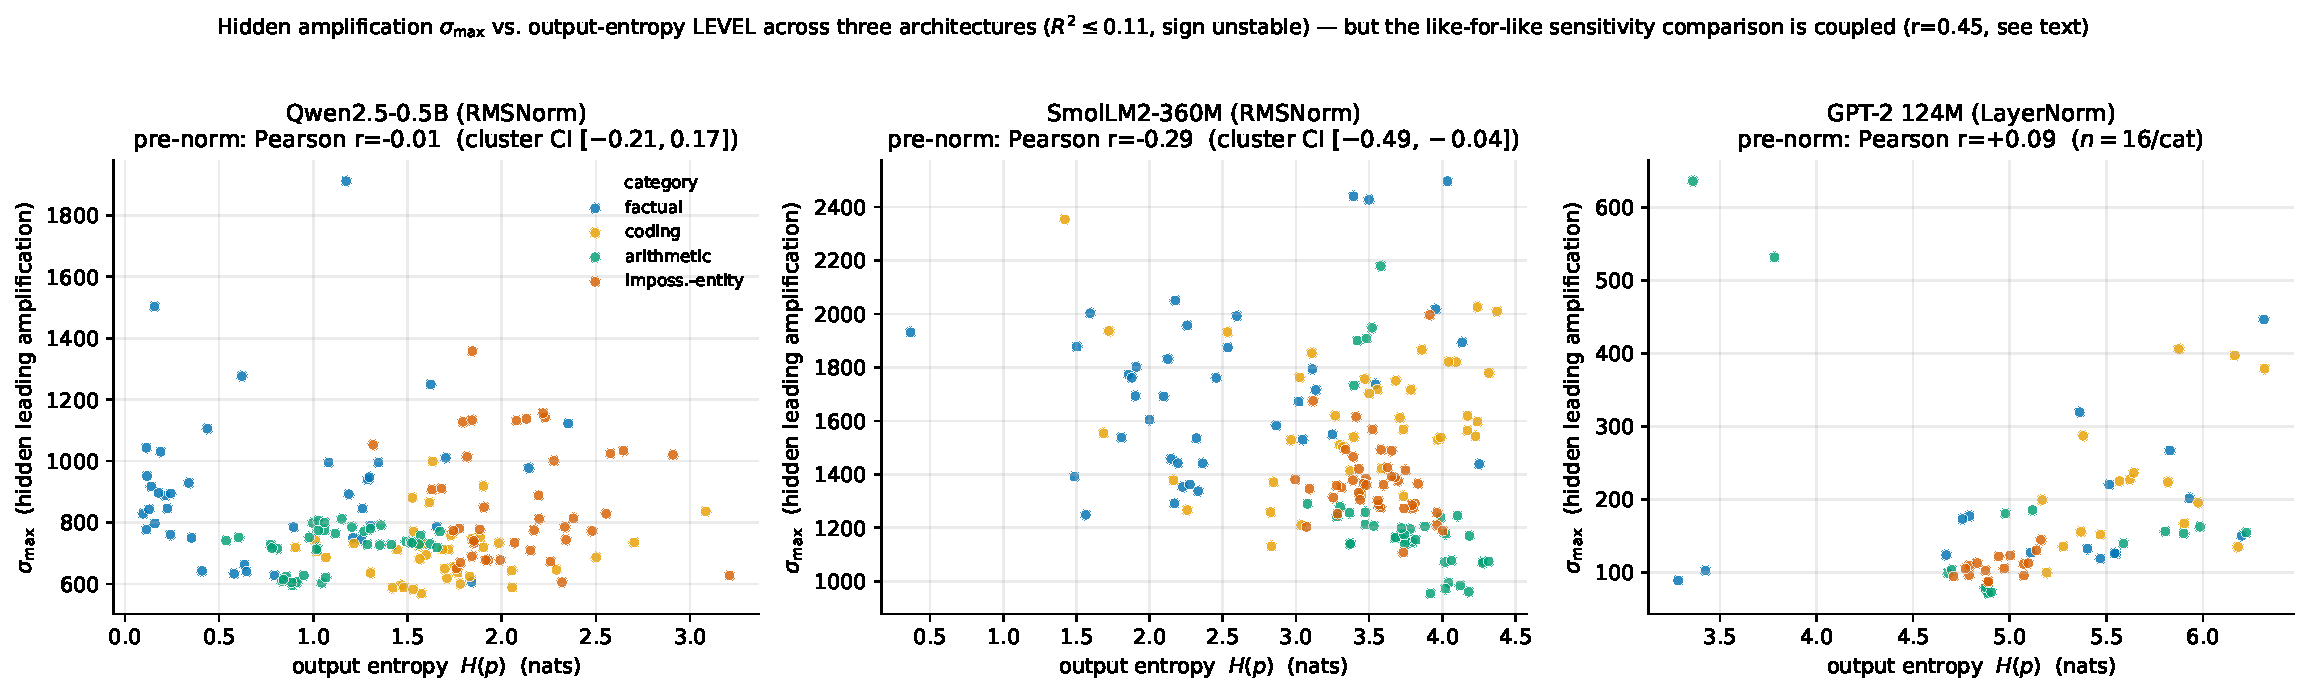
\includegraphics[width=\linewidth]{figures/two_axis_sigma_entropy.pdf}
\caption{The \emph{naive} comparison (Section~\ref{sec:results-inversion}): hidden leading
amplification $\sigma_{\max}$ vs.\ output-entropy \emph{level} $H(p)$, per prompt, across three
architectures --- Qwen2.5-0.5B (RMSNorm, $r=-0.01$), SmolLM2-360M (RMSNorm, $r=-0.29$), GPT-2
(LayerNorm, base model, $n=16$/cat, $r=+0.09$). The near-zero $|r|$ tempts a ``distinct axes''
reading, but it compares a sensitivity to a level; the corrected sensitivity-to-sensitivity
comparison is coupled ($r=0.45$, mostly shared magnitude; Section~\ref{sec:controls},
Figure~\ref{fig:confound}). On the two sub-billion instruction-tuned models factual prompts sit in
the low-entropy, high-$\sigma_{\max}$ corner; that ordering is model-specific (a different class
leads on GPT-2 and $\ge1.5$B; Section~\ref{sec:scale}).}
\label{fig:twoaxis}
\end{figure}

\paragraph{The naive picture is similar on the second model, with model-dependent fine structure.}
The exact-Jacobian profiling for SmolLM2 ($n=40$/category, both read-out sites) reproduces the
\emph{naive} picture and sharpens what is and is not model-invariant --- with the caveat that the
corrected, magnitude-controlled comparison (Section~\ref{sec:controls}) is only the partial
correlation $0.30$ here, so this paragraph describes the level view, not an independence claim. At the
pre-norm site factual is again the \emph{highest}-amplification class ($\sigma_{\max}=1715$, vs.\
coding $1618$, hallucination-prone $1375$, reasoning $1247$) and the \emph{lowest}-entropy class
($2.52$ vs.\ $3.4$--$3.8$), so it again occupies the low-entropy/high-amplification corner. Three
qualifications follow. \emph{(i) The weak level-correlation is not even sign-stable.} On
SmolLM2 the $\sigma_{\max}$--entropy(level) correlation is $r=-0.29$ with a template cluster-bootstrap
$95\%$ CI $[-0.49,-0.04]$ that \emph{excludes} zero, versus $r=-0.01$, CI $[-0.21,0.17]$ on Qwen: the
level correlation is weak on both but small-and-nonzero rather than clean-zero, and its magnitude and
CI are model-dependent ($R^2\le0.09$ throughout). \emph{(ii) Which pairwise contrast survives
clustering is model-dependent.} On SmolLM2 factual $>$ hallucination-prone is cluster-robust
($d=1.40$, cluster permutation $p=0.000$) while factual $>$ coding is not ($d=0.34$, $p=0.19$) --- the
mirror image of Qwen (factual $>$ coding robust, factual vs.\ hallucination-prone underpowered),
matching the model-dependence already seen in Algorithm~1. Neither model establishes factual above
\emph{both} coding and reasoning under clustering. \emph{(iii) The radial reading replicates.} At the
post-norm site factual is no longer the most expansive ($\sigma_{\max}$: coding $88 >$ factual $79 >$
hallucination-prone $75 >$ reasoning $72$; factual vs.\ coding $d=-0.47$), consistent, as on Qwen,
with a radial component removed by RMSNorm. Finally, the Fisher/KL susceptibility $\chi_F$ does
\emph{not} replicate its ordering across models (its category ranking and even the sign of its
correlation with entropy differ, $+0.49$ on Qwen vs.\ $-0.20$ on SmolLM2), further supporting our
treatment of $\chi_F$ as an output-side, entropy-related measure rather than a stable axis.

The level view is the same on the sampled-direction metric across \emph{both} models: factual
prompts are simultaneously the most output-confident (lowest $H(p)$, highest $p_{\max}$) and the
largest in finite-depth response $\lambda_L^{(\epsilon)}$. Relative to factual, hallucination-prone
prompts differ by $d\approx-2.0$ in entropy but by only $d=+0.09$ (Qwen) or $+0.99$ (SmolLM) in
$\lambda_L^{(\epsilon)}$; reasoning prompts differ by $d\approx-2.0$ in entropy yet by $d=+1.1$
(Qwen) to $+2.4$ (SmolLM) in $\lambda_L^{(\epsilon)}$. This wide separation on the entropy
\emph{level} is exactly the pattern Section~\ref{sec:controls} shows to be misleading when read as
axis-independence: it contrasts a level against a sensitivity. We explicitly do \emph{not} claim
hallucination-prone prompts are the maximum of hidden amplification (pre-norm, factual prompts are),
and we do \emph{not} treat the Fisher/KL susceptibility $\chi_F$ as a third axis: as shown in
Section~\ref{sec:results-alg2} it partially tracks entropy.

\subsection{Controls: what the near-zero correlation does and does not mean}
\label{sec:controls}
The near-zero correlation between $\sigma_{\max}$ and output entropy is easy to over-read as
``independent axes.'' It is not, and the analysis is instructive --- it is the main lesson of
this case study. All tests below are on the Qwen $n=40$/category data (forward passes; one backward
per prompt for the gradient test; the geometric-alignment check additionally reuses the Algorithm~2
leading singular vector $v_{\mathrm{lead}}$).

\paragraph{The correct comparison is sensitivity-to-sensitivity, and the coupling is mostly magnitude.}
$\sigma_{\max}$ is a hidden-state \emph{sensitivity}; output entropy $H(p)$ is a \emph{level}. Their
near-zero correlation ($r=-0.01$; $r=-0.11$ once the quarantined reasoning class is excluded;
post-norm $r=-0.06$) partly just reflects that mismatch, and even it hides weak nonlinear structure
(distance correlation $0.20$; a within-category, centroid-removed value and a permutation $p$ are
reported in Appendix~\ref{sec:robustness}). The like-for-like comparison uses the entropy's
\emph{input sensitivity} $\|\nabla_{H_0}H(p)\|$ (one backward per prompt): the Pearson correlation
$r(\|\nabla_{H_0}H\|,\sigma_{\max})=0.45$ on Qwen ($n=160$). But this is largely \emph{shared
Jacobian magnitude}, not a specific coupling: partialling out the bulk norm $\lambda_{\mathrm{bulk}}$
reduces the partial correlation
$r(\|\nabla_{H_0}H\|,\sigma_{\max}\mid\lambda_{\mathrm{bulk}})$ to $0.10$ (bootstrap $95\%$ CI
$[-0.09,0.29]$). Replicated with one backward per prompt on the other models, the partial correlation
is $0.30$ (SmolLM2, $n=160$, CI $[0.16,0.44]$) and $0.30$ (GPT-2, $n=64$, CI $[-0.27,0.61]$ --- barely
more than a sign at this $n$); on two of the three models the residual CI includes zero, so the
magnitude-controlled coupling is \emph{weak and model-dependent} ($0.10$--$0.30$, $\mathrm{R}^2\le0.09$).

We pre-empt the obvious objection --- that partialling a covariate $0.80$-correlated with
$\sigma_{\max}$ mechanically shrinks the partial, so the drop is collinearity arithmetic rather than
evidence of shared magnitude. It is the shared magnitude: $\lambda_{\mathrm{bulk}}$ is shown
independently to drive \emph{both} sides. It is $r=0.80$-correlated with $\sigma_{\max}$ \emph{and}
$r(\|\nabla_{H_0}H\|,\lambda_{\mathrm{bulk}})=0.50$ on Qwen ($0.27$ SmolLM2, $0.38$ GPT-2) --- on Qwen
the entropy sensitivity tracks the bulk norm \emph{more} tightly than it tracks $\sigma_{\max}$ itself
($0.50>0.45$). So a single common scale (big Jacobians are big everywhere) sits behind the raw $0.45$,
and removing it is removing a real common cause, not manufacturing a null. We report this
decomposition, not a single number.

\paragraph{A collinearity-free check: the directions are partially aligned.}
Partialling removes a covariate correlated with $\sigma_{\max}$, so a skeptic could call the drop
mechanical. As an independent check that involves no partialling, we compare the two input directions
\emph{geometrically}. Let $v_{\mathrm{lead}}$ be the leading right singular vector of the hidden
Jacobian $J$ (the input-embedding direction most amplified into the final pre-norm hidden state;
Algorithm~2) and $\nabla_{H_0}H$ the entropy input-gradient (the direction that most increases output
entropy; one backward). Both live in the same $T\times d$ input space, so their angle is well defined.
Over the Qwen $n=160$ prompts the mean absolute cosine is
$|\!\cos\angle(\nabla_{H_0}H,v_{\mathrm{lead}})|=0.41$ (median $0.37$). Because both vectors concentrate
their energy on the last token positions, the fully-random null $\sqrt{2/(\pi N)}\approx0.0046$
($N=T\!\cdot\!d\approx3\times10^4$) understates chance; the honest comparison is a
\emph{position-matched} null --- random directions carrying $\nabla_{H_0}H$'s per-position energy
profile --- which raises the null only to $0.008$ (Monte-Carlo and closed form agree). Against it
$|\!\cos|=0.41$ is still $\approx\!53\times$ chance, and $97.5\%$ of prompts exceed their own
position-matched null, so the alignment is genuine \emph{within}-position directional structure, not a
positional-support artifact. The two directions are thus \emph{not} orthogonal. But the alignment is
partial, not dominant ($\overline{\cos^2}=0.24$: about three-quarters of the entropy-sensitivity
direction lies \emph{outside} the leading stretch direction), and it is largest for
hallucination-prone prompts ($0.55$, consistent with the along-$v_{\mathrm{lead}}$ susceptibility of
Section~\ref{sec:results-alg2} and, like it, partly entropy-related). The two analyses agree on an intermediate
picture: \emph{across} prompts the magnitude co-variation is dominated by a common scale (partial
correlation $0.1$--$0.3$), while \emph{within} a prompt the hidden-amplification and output-sensitivity
directions share a real but modest overlap. Neither ``independent axes'' nor ``strongly coupled'' is
accurate --- and that the partial correlation ($0.10$) and the direct geometry ($\cos^2=0.24$) read
differently is itself the methodological point: no single summary is safe to read alone.

\paragraph{The leading value is largely redundant with the bulk.}
With stable rank $\approx4$ in $d\approx900$, $\sigma_{\max}^2\approx\|J\|_F^2/4$, and indeed the
per-prompt correlation between the leading amplification and the bulk prediction is
$r(\sigma_{\max},\lambda_{\mathrm{bulk}})=0.80$. For the categorical contrast the exact leading value
adds little over the cheap sampled-direction/bulk statistic; Algorithm~2's value is in the
anisotropy, directions, and output-side operators, not in $\sigma_{\max}$ alone.

\paragraph{$\sigma_{\max}$ is not hidden-state norm, nor prompt surprise.}
$\sigma_{\max}$ correlates only moderately with the final-token hidden-state norm $\|h_{L,T}\|$
($r=0.38$, $\mathrm{R}^2=0.15$) and not at all with the language-model perplexity of the prompt
($r=-0.01$). Controlling for $\|h_{L,T}\|$, the factual-vs-coding contrast shrinks but survives
($d=1.12\to0.80$). So the finding is not a re-description of norm inflation or of an ``easy'' prefix.

\paragraph{A linear probe already separates the categories --- which is the point.}
A logistic probe on the raw final hidden state ($\ell_2$-regularized, $C=1$, standardized features;
$n=160$, $d=896$, so $n\!\ll\!d$) separates the four categories at $99\%$ (5-fold CV; chance $25\%$).
By contrast, a probe on our \emph{four spectral scalars}
$(\sigma_{\max},\lambda_{\mathrm{bulk}},r_{\mathrm{stable}},\chi_F^{\max})$ reaches only
$54\%$, and one on $(\|h_\text{pre}\|,\|h_\text{post}\|,\text{ppl})$ reaches $66\%$: the spectral
observables carry \emph{some} categorical signal (well above the $25\%$ chance) but far less than the
full hidden state, quantifying that they are low-dimensional summaries, not classifiers. Category
identity is trivially decodable from $h_{L,T}$, so we do \emph{not} propose the spectral observables as
classifiers. Their content is the \emph{correlation structure} between response geometry and output
uncertainty --- the level-vs-sensitivity and magnitude decomposition above --- which a supervised
category probe does not provide.

\paragraph{The output-uncertainty signal is not a single-token artifact.}
Replacing the first-token entropy with the mean entropy over the first eight \emph{generated} tokens
(greedy) leaves hallucination-prone prompts the outlier (halluc-vs-others $|d|=0.9$--$2.1$, vs.\
$1.0$--$2.9$ single-token; correlation $0.65$), so the output axis is not an artifact of the chat
template's near-deterministic first token. We nonetheless read the output axis as close to a
manipulation check: impossible-entity prompts have diffuse continuations largely by construction.

\subsection{Exact-Jacobian validation (Algorithm 2)}
\label{sec:results-alg2}

We profile the exact input$\to$final-token Jacobian on \textbf{Qwen2.5-0.5B} at $n=40$
prompts/category (both read-out sites, $160$ prompts each). The $40$ are the first $40$ per category
in the length-matched set's fixed generation order (a deterministic, seed-independent draw); this
subset preserves the exact token-length matching of the full set (identical per-category $T$
histograms, Kruskal--Wallis $p=1.000$; Appendix~\ref{sec:robustness}), so it introduces no length
confound. We use $n_{\mathrm{iter}}=15$ (median
convergence residual $4\times10^{-4}$; $5\%$ of prompts above $10^{-2}$). This is our exact-Jacobian
profiling at both read-out sites on Qwen; the SmolLM2 profiling, \emph{also at both read-out sites}
and showing the same weak $\sigma_{\max}$--entropy-level pattern, is reported in
Section~\ref{sec:results-inversion} (post-norm in Section~\ref{sec:results-inversion}(iii)). Only the
intermediate-scale sanity check (Section~\ref{sec:scale}) is an offline follow-up. The
significance bar is the Holm-adjusted permutation $p$ (with cluster-aware inference below), and every
number in this subsection is a mean over $n=40$ prompts/category on Qwen.

\paragraph{Pre-norm: factual leads the hidden axis, under cluster-aware inference.}
At the pre-norm read-out the leading amplification $\sigma_{\max}$ is largest for factual ($914.7$)
and lowest for coding ($704.3$), with hallucination-prone ($865.3$) and reasoning ($717.3$) between
(Figure~\ref{fig:box}, left). Because templated prompts are near-duplicates, we judge significance by
\emph{cluster} permutation on the template id (distinct templates per category: factual $39$, coding
$40$, hallucination-prone $28$, reasoning only $5$). Factual $>$ coding is large and cluster-robust
($d=1.12$; cluster permutation $p=0.000$; cluster-bootstrap $95\%$ CI of the mean difference
$[+133,+297]$). Factual $>$ reasoning is also large ($d=1.08$) but is \emph{not} cluster-robust
(cluster permutation $p=0.11$), because the reasoning class is backed by only five templates; we
report it as suggestive, not established. Factual and hallucination-prone are statistically
indistinguishable ($d=0.22$, cluster permutation $p=0.35$), and equivalence testing does \emph{not}
license calling them equal: two one-sided tests (TOST) at a $\pm0.5$\,SD margin are non-significant
($p=0.29$), so this contrast is \emph{underpowered} --- neither a difference nor a demonstrated
equivalence, and we avoid the language of a ``tie''. The bulk identity is borne out
(Figure~\ref{fig:bulk}): the sampled statistic tracks $\lambda_{\mathrm{bulk}}$ with median relative
error $3.3\%$ (Pearson $r=0.79$, $n=160$), confirming the single-random-direction protocol realizes
the bulk Jacobian statistic. The Jacobian anisotropy is largest for factual (lowest stable rank,
$r_{\mathrm{stable}}=3.50$ vs.\ $3.6$--$4.5$; Figure~\ref{fig:box}, middle), cluster-robust against
coding but --- like every reasoning-involving contrast --- not cluster-robust against the
low-diversity reasoning class.

\begin{figure}[t]\centering
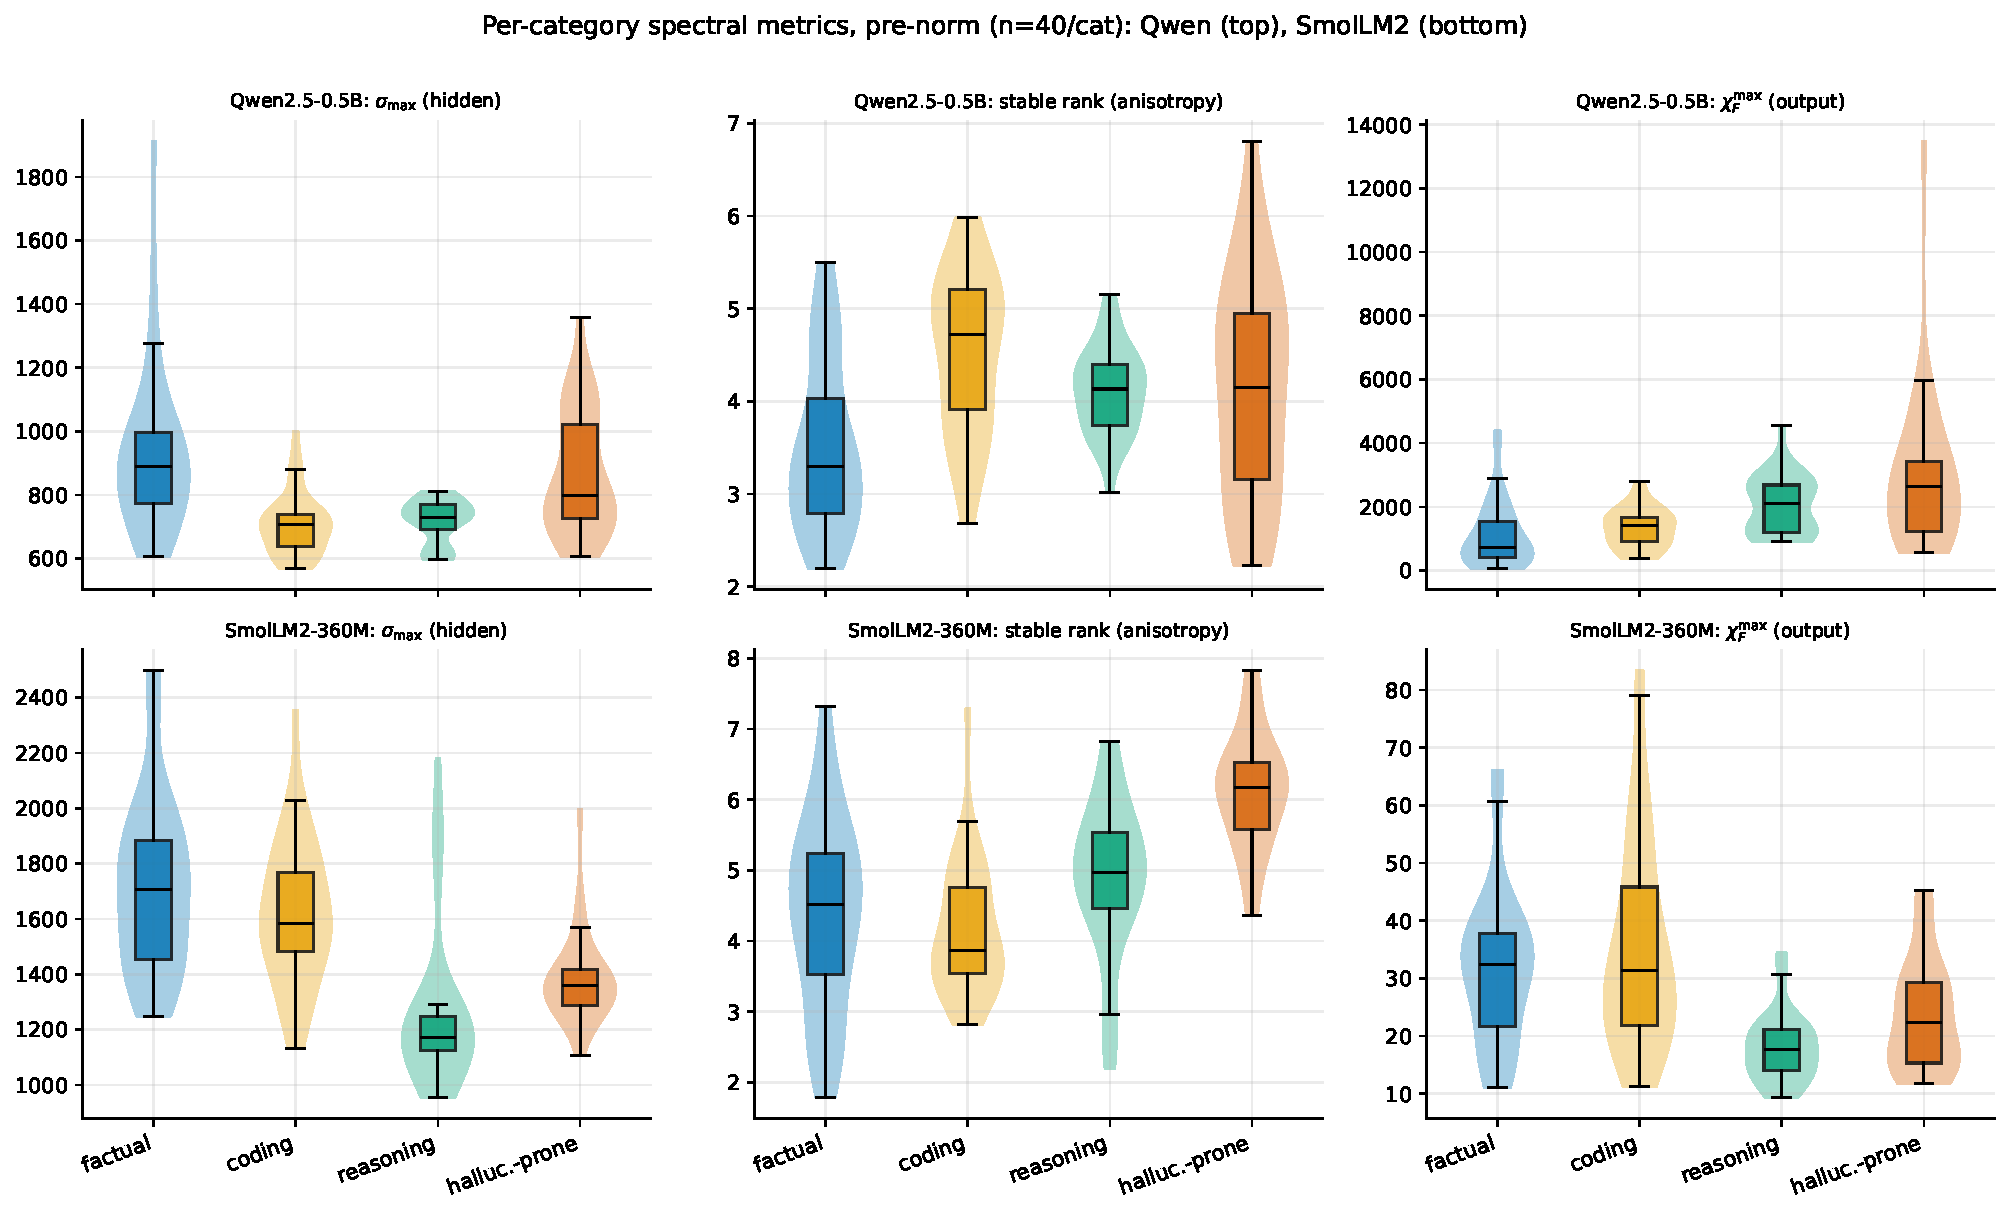
\includegraphics[width=\linewidth]{figures/box_spectral_metrics.pdf}
\caption{Per-category spectral metrics, pre-norm ($n=40$/category), for both models: Qwen2.5-0.5B
(top row), SmolLM2-360M (bottom row); per-panel $y$-scales differ across models. Hidden amplification
$\sigma_{\max}$ (left) and anisotropy (stable rank, middle) place factual high/low respectively on
both models, whereas the output-distribution susceptibility $\chi_F^{\max}$ (right) does not order the
categories consistently across models --- it partly tracks output entropy (Figure~\ref{fig:confound})
and is not an independent axis. None of these summaries is independent of output uncertainty once
compared like-for-like (Section~\ref{sec:controls}).}
\label{fig:box}
\end{figure}

\begin{figure}[t]\centering
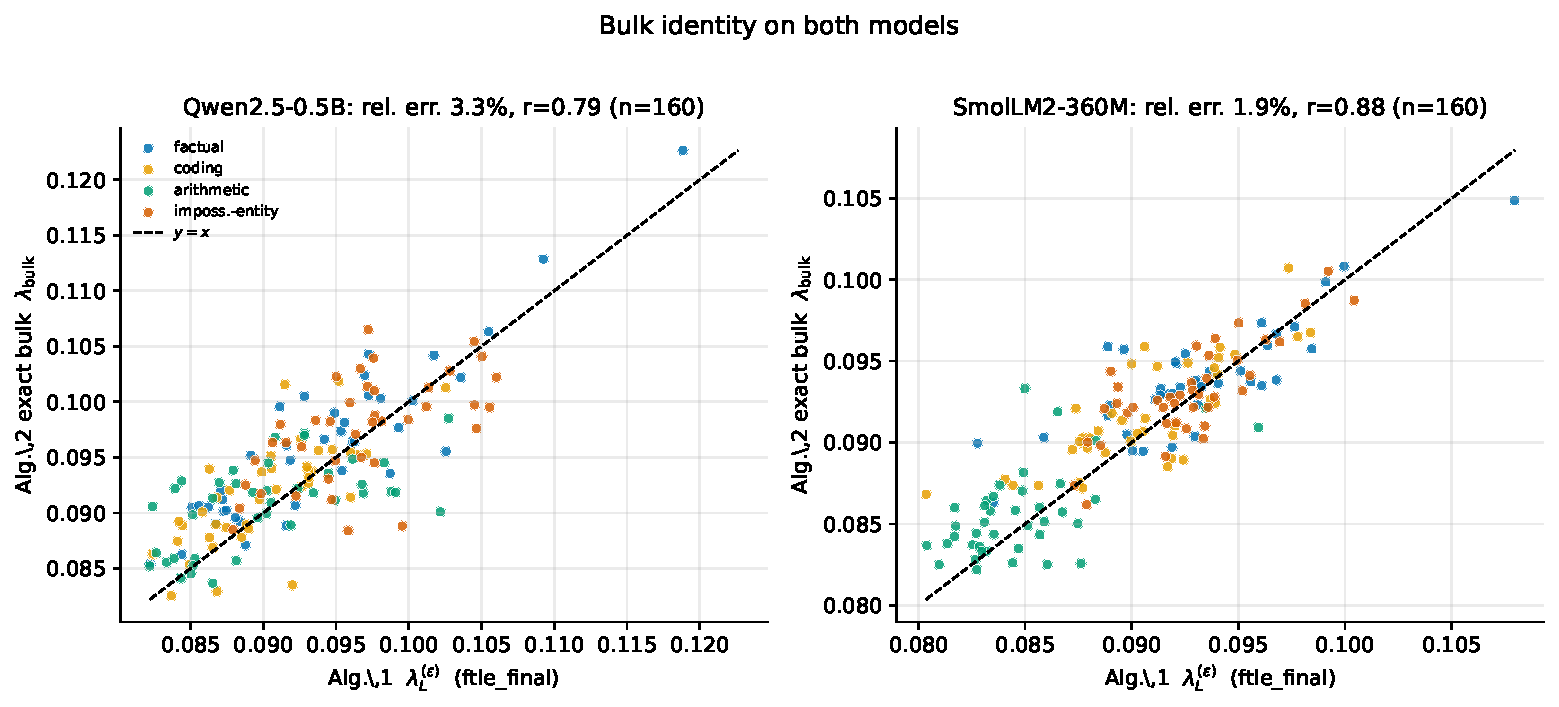
\includegraphics[width=\linewidth]{figures/bulk_identity.pdf}
\caption{The bulk identity on both models: the Algorithm-1 sampled-direction statistic
$\lambda_L^{(\epsilon)}$ (\texttt{ftle\_final}) against the Algorithm-2 exact bulk prediction
$\lambda_{\mathrm{bulk}}=\tfrac1{2L}\log(\|J\|_F^2/N)$, per prompt ($n=160$ each). Points track the
$y{=}x$ line with median relative error $3.3\%$ (Pearson $r=0.79$) on Qwen and $1.9\%$ ($r=0.88$) on
SmolLM2; the small systematic offset is the Jensen bias discussed in the text. The identity
replicates on both models.}
\label{fig:bulk}
\end{figure}

\paragraph{Fisher/KL susceptibility tracks entropy, with an analytic reason.}
That $\chi_F$ should track entropy is not a surprise but has an analytic skeleton. Since
$\chi_F^{\max}=\tfrac12\lambda_{\max}(J_z^\top F J_z)\le\tfrac12\lambda_{\max}(F)\,\sigma_{\max}(J_z)^2$,
and the Fisher matrix $F=\mathrm{diag}(p)-pp^\top$ has $\lambda_{\max}(F)\to0$ at \emph{both} entropy
extremes --- $\lambda_{\max}(F)\to0$ as $p\to$ one-hot (minimum entropy) and $\lambda_{\max}(F)=O(1/|\mathcal V|)$
as $p\to$ uniform (maximum entropy) --- the $F$-factor is a non-monotone, entropy-dependent envelope.
$\chi_F$ thus inherits an entropy dependence through $F$ on top of the input-Jacobian factor
$\sigma_{\max}(J_z)$, and its \emph{sign} of correlation with entropy depends on which side of the
envelope a model's operating distribution sits --- consistent with the flip we observe ($r=+0.49$ on
Qwen, $-0.20$ on SmolLM2) and with the $\sim\!10^3$ vs.\ $\sim\!10^1$ scale difference (larger
vocabulary and logit scale push $\lambda_{\max}(F)$ and $\sigma_{\max}(J_z)$ differently). Empirically:
$\chi_F^{\max}$ ranks factual \emph{lowest} ($1111$) and hallucination-prone \emph{highest} ($2849$),
reasoning ($2045$) and coding ($1330$) between (Figure~\ref{fig:box}, right). This ordering is
\emph{not} independent of the output-uncertainty axis. Across the $n=160$ prompts, $\chi_F^{\max}$ correlates with output entropy
at Pearson $r=0.49$ (Spearman $0.56$), and when we regress $\chi_F$ on entropy and top-1 probability
and test the category structure on the residuals, the factual-vs-hallucination contrast collapses
from $d=-0.98$ to $d=-0.19$ (residual permutation $p=0.46$; Figure~\ref{fig:confound}). The factual/
hallucination separation on $\chi_F$ is thus largely a re-expression of their entropy difference.
We therefore \emph{do not} treat $\chi_F$ as an independent observable. It remains useful for a
different reason: unlike the entropy of a static distribution, $\chi_F$ links an \emph{input
perturbation} to \emph{movement} of the output distribution, and its residuals retain some
non-entropy structure (a coding-vs-reasoning contrast). We report it as an output-side,
entropy-related susceptibility, not an independent axis. The hidden amplification $\sigma_{\max}$ is
likewise not an independent axis: it is only weakly related to the entropy \emph{level} but
moderately coupled to the entropy's input \emph{sensitivity} (Section~\ref{sec:controls}); the
summary is that these Jacobian quantities are correlated mainly through shared magnitude.

\begin{figure}[t]\centering
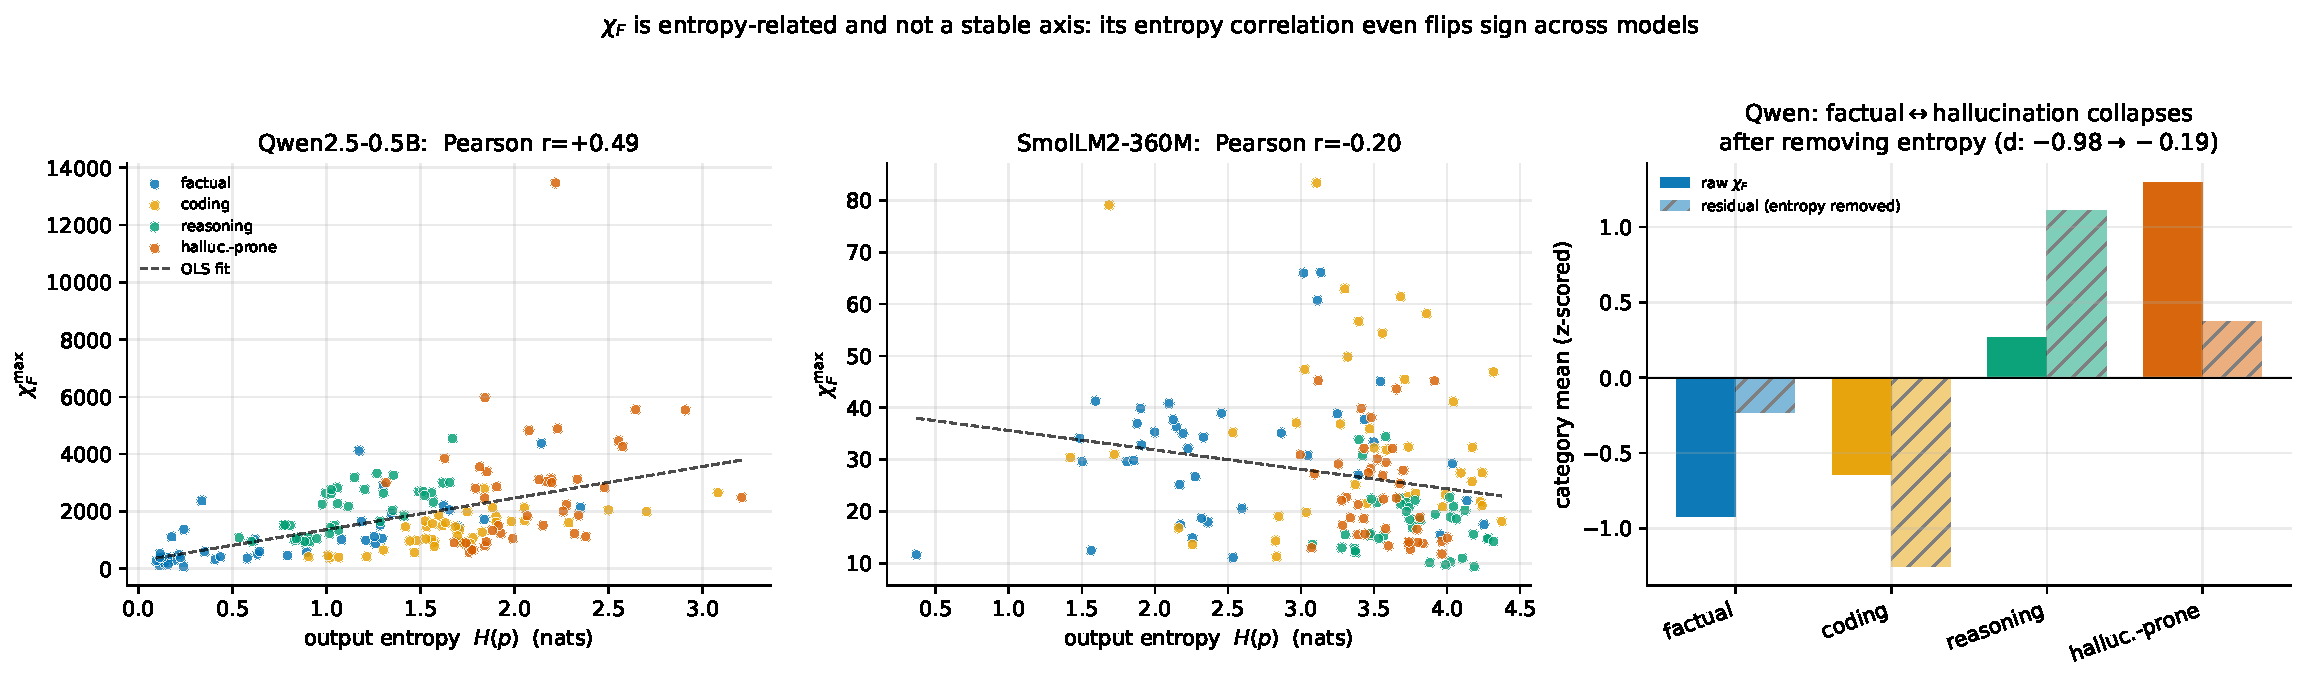
\includegraphics[width=\linewidth]{figures/chiF_entropy_confound.pdf}
\caption{$\chi_F$ is entropy-related and not a stable axis (pre-norm, $n=160$/model). Left and
middle: $\chi_F^{\max}$ vs.\ output entropy on Qwen (Pearson $r=+0.49$) and SmolLM2 ($r=-0.20$) --- the
correlation even \emph{flips sign} across models, so $\chi_F$ is not a stable output-side axis. Right
(Qwen): category means of $\chi_F$ (z-scored), raw vs.\ residual after regressing out entropy and top-1
probability; the factual$\leftrightarrow$hallucination ordering collapses (Cohen $d$: $-0.98\to-0.19$,
$p=0.46$), while a residual coding/reasoning contrast remains.}
\label{fig:confound}
\end{figure}

\paragraph{Post-norm: the hidden ordering is consistent with a radial component.}
At the post-norm read-out (after the final RMSNorm) the hidden axis changes: factual is no longer
the most expansive. The post-norm $\sigma_{\max}$ ordering is reasoning ($5634$) $>$
hallucination-prone ($5256$) $>$ factual ($4840$) $>$ coding ($4447$), and factual is now
significantly \emph{below} reasoning ($d=-0.67$, Holm $p=0.014$) rather than above it
(Figure~\ref{fig:prepost}). The final RMSNorm rescales the hidden state to unit root-mean-square,
removing its radial component \cite{zhang2019root}; the pre-versus-post reversal is therefore
\emph{consistent with} factual's excess pre-norm amplification lying largely along the radial
direction, though we do not claim a definitive decomposition, as the two read-out sites also differ
in the last block's transformation. We read only the pre$\to$post \emph{reordering}, not the absolute
scale: the overall $\sigma_{\max}$ magnitude moves in \emph{opposite} directions across models
(pre$\to$post rises $\sim\!5\times$ on Qwen but falls $\sim\!20\times$ on SmolLM2;
Figure~\ref{fig:prepost}), because RMSNorm's rescaling folds in a model-specific learned gain $\gamma$
and RMS level. That absolute change is uninterpreted; only which class \emph{leads} carries the radial
reading, and the class-leadership reshuffle is the same (factual loses its lead) on both. The output
response $\chi_F$ is, as expected, identical between
the two sites (it depends on the logits, not the tracked hidden index), so the output-distribution
ordering is norm-invariant, whereas the hidden-state ``factual is most
expansive'' statement holds only pre-norm and is representation-dependent --- which tempers any
reading of factual as internally the most perturbation-expansive class.

\begin{figure}[t]\centering
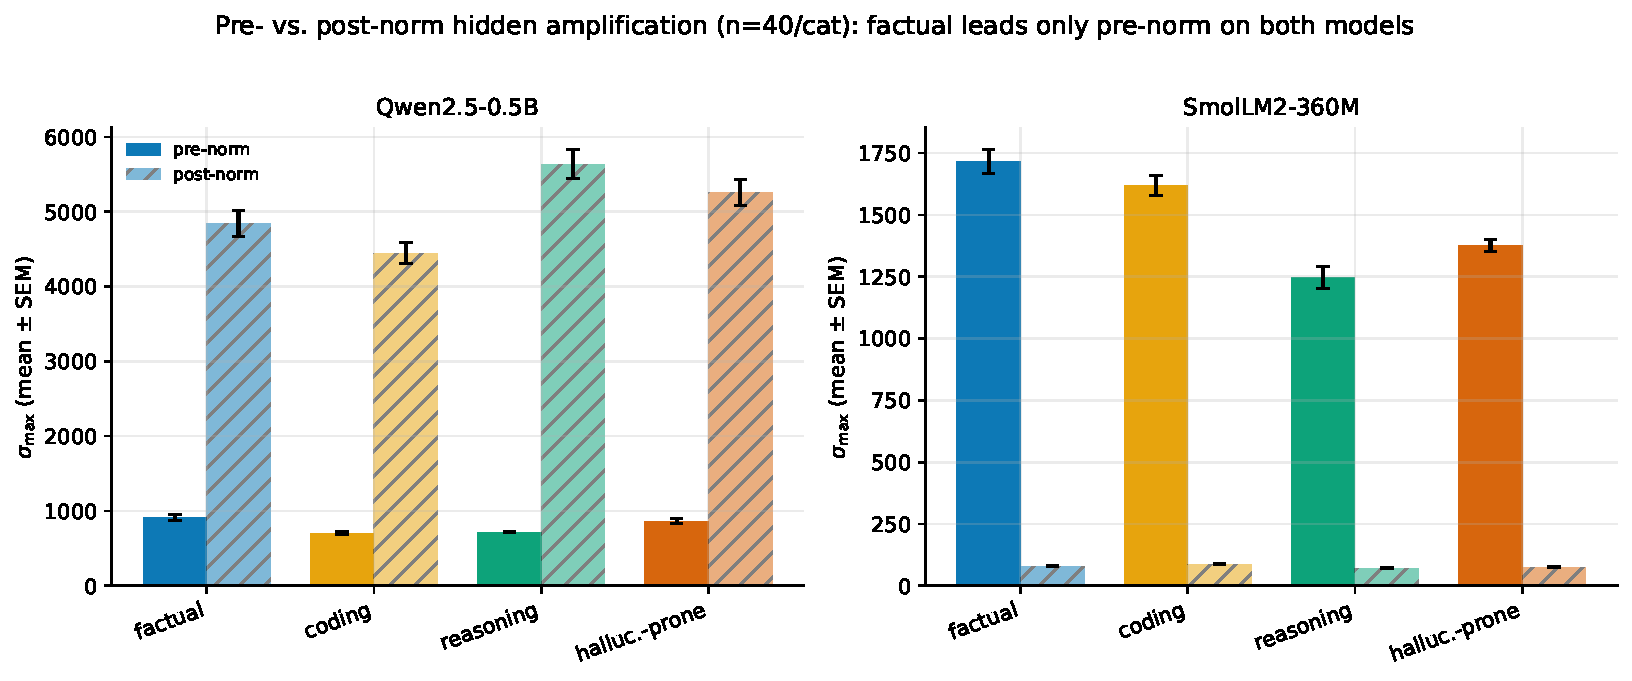
\includegraphics[width=\linewidth]{figures/pre_post_norm_shift.pdf}
\caption{Pre- vs.\ post-norm hidden amplification $\sigma_{\max}$ (mean $\pm$ SEM, $n=40$/category)
for both models: Qwen2.5-0.5B (left), SmolLM2-360M (right); per-panel $y$-scales differ, and the
absolute pre$\to$post change is opposite across models ($\sim\!5\times$ up on Qwen, $\sim\!20\times$
down on SmolLM2 --- a model-specific final-norm gain, uninterpreted; see text). On both,
factual leads only at the pre-norm site and the ordering rearranges post-norm, consistent with a
radial component removed by RMSNorm.}
\label{fig:prepost}
\end{figure}

\paragraph{Mechanism (secondary, and also entropy-related).}
The hidden leading direction moves the output more for hallucination-prone than for other classes:
$\chi_F$ evaluated along $v_{\mathrm{lead}}$ is highest for hallucination-prone (vs.\ factual
$d=-0.86$, coding $d=-0.91$, reasoning $d=-0.79$). We flag this as secondary rather than a headline,
for two reasons. First, this along-lead susceptibility itself correlates with output entropy
($r=0.42$), so it inherits the confound of the previous paragraph. Second, the direction-overlap
$\alpha$ between the hidden-stretch and output-moving directions is largest for hallucination-prone
but significantly so only against coding and reasoning, not factual ($d=-0.51$, Holm $p=0.077$), and
these reasoning contrasts are not cluster-robust. The gap is thus driven more by hallucination-prone's
globally higher output sensitivity (which tracks entropy) than by a distinctive alignment. We
explicitly do \emph{not} claim factual is ``output-orthogonal'' --- that claim does not survive at
$n=40$.

\begin{table}[t]\centering\small
\begin{tabular}{llrrrr}
\toprule
Read-out & Model & $n$/cat & $\sigma_{\max}$ order (hidden) & $\chi_F^{\max}$ order (output) & bulk rel.\ err. \\
\midrule
pre-norm  & Qwen2.5-0.5B & 40 & fac $>$ cod (c.r.); fac $>$ rea (n.\,c.r.) & hal$>$rea$>$cod$>$fac & $3.3\%$ \\
post-norm & Qwen2.5-0.5B & 40 & rea$>$hal$>$fac$>$cod & hal$>$rea$>$cod$>$fac & --- \\
pre-norm  & SmolLM2-360M & 40 & fac $>$ hal (c.r.); fac $\approx$ cod (n.\,c.r.) & cod$>$fac$>$hal$>$rea & $1.9\%$ \\
post-norm & SmolLM2-360M & 40 & cod$>$fac$>$hal$>$rea & cod$>$fac$>$hal$>$rea & --- \\
\bottomrule
\end{tabular}
\caption{Algorithm-2 exact-Jacobian profiling, both models, both read-out sites ($n=40$/category,
$n_{\mathrm{iter}}=15$; numerical self-test PASS). ``c.r.''/``n.\,c.r.'' = cluster-robust / not
cluster-robust under template-level permutation. On \emph{both} models factual has the highest
pre-norm $\sigma_{\max}$ and the lowest entropy, but \emph{which} pairwise contrast survives
clustering is model-dependent: factual $>$ coding on Qwen ($p=0.000$) vs.\ factual $>$
hallucination-prone on SmolLM2 ($p=0.000$); reasoning-involving contrasts are never cluster-robust
(only five reasoning templates), and factual vs.\ hallucination-prone on Qwen is underpowered, not
equal. At the post-norm site factual is no longer the most expansive on either model, consistent
with a radial component removed by the final RMSNorm. The bulk identity replicates (Qwen rel.\ err.\
$3.3\%$, $r=0.79$; SmolLM2 $1.9\%$, $r=0.88$); the ``---'' in the post-norm bulk column marks that the
Algorithm-1 identity is defined only at the pre-norm site it tracks, so no post-norm bulk error is
computed. The output ordering $\chi_F^{\max}$ is
representation-independent on the output side but partially tracks entropy and does \emph{not}
replicate across models (Section~\ref{sec:results-alg2}, Figure~\ref{fig:confound}); it is not an
independent axis. Algorithm-1 results for both models are in Table~\ref{tab:lm-dynamics}; the
intermediate-scale check is Section~\ref{sec:scale}.}
\label{tab:alg2}
\end{table}

\subsection{Intermediate-scale sanity check}
\label{sec:scale}
A natural objection is that both primary models are sub-billion and might not represent larger
Transformers. Because Algorithm~2 is expensive (Section~\ref{sec:methods-cost}), a full sweep at
larger scale is not affordable here; instead we run a deliberately \emph{minimal} sanity check on
two intermediate-scale models, Qwen2.5-1.5B-Instruct and Qwen2.5-3B-Instruct (both instruction-tuned,
matching our primary models --- so the check varies scale, not the instruction-tuning axis), as an offline follow-up to the main
sweep. The configuration is reduced across every axis --- $n{=}8$ prompts/category, pre-norm
read-out only, block size $k{=}3$, $6$ sphere probes, $8$ subspace iterations, Fisher enabled ---
and writes to a separate directory with the same checkpointing (per-row flush, resume by
$(\text{model},\text{index},\text{category},\text{prompt index})$, per-run manifest with hardware
and completed/failed counts). Because the Qwen2.5 family shares one tokenizer, the length-matched
prompt set built for Qwen2.5-0.5B is length-matched for these models too and is reused unchanged.
This check is emphatically \emph{not} a scaling result: with $n{=}8$/category it can only indicate
whether the qualitative patterns of Sections~\ref{sec:results-alg2} --- the weak $\sigma_{\max}$--entropy
level correlation, and the factual-high-$\sigma_{\max}$ ordering --- are present beyond sub-billion
models. We \emph{pre-specify} three readings of the outcome (stated here, before the check, and
applied unchanged in the Discussion; there is no external pre-registration):
\emph{(i)} both the smallness of the level correlation \emph{and} the factual-high-$\sigma_{\max}$
ordering persist, which would argue for generality; \emph{(ii)} the smallness of the level correlation
persists but the specific category ordering does not, which would mark Algorithm~2 as a diagnostic and
the factual-corner ordering as sub-billion-specific; \emph{(iii)} neither persists, which would make
the whole pattern a sub-billion artifact. None of the three upgrades the naive level statistic into
axis-independence: that question is settled only by the magnitude-controlled comparison of
Section~\ref{sec:controls}, which we ran at $0.5$B and did not repeat here.
\IfFileExists{figures/scale_sanity.pdf}{%
\begin{figure}[t]\centering
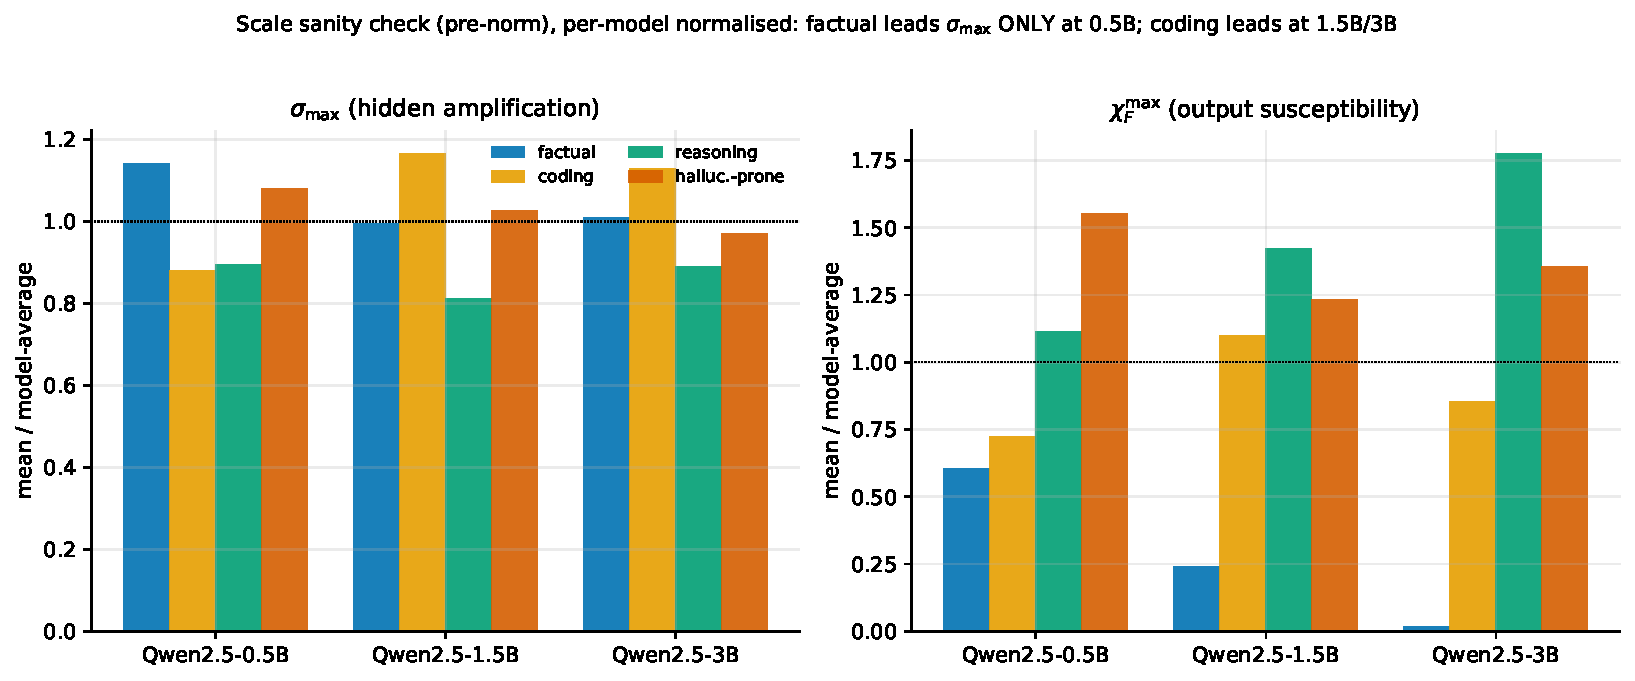
\includegraphics[width=\linewidth]{figures/scale_sanity.pdf}
\caption{Scale-sanity check (pre-norm; $n=40$/category for $0.5$B, $n=8$/category for $1.5$B/$3$B):
per-category means of hidden amplification $\sigma_{\max}$ (left) and output susceptibility
$\chi_F^{\max}$ (right) for Qwen2.5-0.5B/1.5B/3B, each \emph{normalised to its own model-average}
(dotted line $=1$) because absolute scales differ across models; read the within-model ordering.
Factual (blue) leads $\sigma_{\max}$ \emph{only} at $0.5$B; at $1.5$B and $3$B coding (yellow) leads,
so the factual-highest result does not persist beyond sub-billion. The $\chi_F$ ordering is itself
inconsistent across scales (hallucination-prone highest at $0.5$B, reasoning at $1.5$B/$3$B),
reinforcing its demotion. A qualitative sanity check ($n=8$), not a scaling law.}
\label{fig:scale}
\end{figure}}{}%
\paragraph{Outcome.} The check gives a \emph{split} result (Figure~\ref{fig:scale}). What is stable:
the weak $\sigma_{\max}$--entropy-level correlation persists ($r=+0.32$ and $-0.01$ at $1.5$B/$3$B, as
$-0.01$ at $0.5$B; $\mathrm{R}^2\le0.10$ throughout), and factual remains the \emph{lowest}-entropy
class at all three scales ($H(p)=0.79,0.29,0.00$). We caution that this is the \emph{naive} summary;
the corrected sensitivity-to-sensitivity, magnitude-controlled comparison (Section~\ref{sec:controls})
was performed only on Qwen-0.5B and should not be assumed to scale. What does \emph{not} persist: the
sub-billion ordering that \emph{factual} has the highest pre-norm $\sigma_{\max}$ --- at both $1.5$B
and $3$B the highest-amplification class is \emph{coding} (factual second). The $\chi_F$ ordering is
likewise scale-inconsistent. So both the category ordering \emph{and} the sign of the weak
level-correlation are model-dependent; only the smallness of that correlation is stable. With
$n{=}8$/category this is a sanity check, not a powered result; scripts and per-model resource
estimates for a fuller validation are provided with the code.

\paragraph{A second architecture: LayerNorm.}
Because our narrative involves the final normalization, we also profile GPT-2 (124M, classic
\emph{LayerNorm}, a base non-instruct model \cite{radford2019language}; $n=16$/category), verifying that final\_index $=-1$ is the
true post-norm readout state ($\mathrm{lm\_head}(h_{-1})=\text{logits}$, as for the RMSNorm models).
Being a base model, GPT-2 has no chat template, so the raw prompt string is tokenized with its native
byte-level BPE and fed directly --- the same convention across Algorithm~1, Algorithm~2, and the
gradient test, so no template tokens enter the perturbed input. Length matching is redone on GPT-2's
own BPE (a separate length-matched set, its own per-category $T$ histograms), so the shorter,
no-template encodings do not reintroduce a length confound.
The \emph{level} comparison behaves as on the RMSNorm models: $\sigma_{\max}$ is weakly correlated
with the entropy level both pre- and post-norm ($r=+0.09$ and $+0.05$, $n=64$; no CI at this $n$), so
the smallness of the level-correlation is not specific to RMSNorm or instruction tuning. The
magnitude-controlled comparison of Section~\ref{sec:controls} gives a partial correlation of $0.30$
here too ($n=64$, wide CI; the residual coupling is weak and model-dependent on all three models). The
pre/post-norm
\emph{reshuffle}, by contrast, cannot be tested here: as on the $1.5$B/$3$B models, factual is not the
highest-amplification class on GPT-2 (coding leads at both sites), so there is no factual lead to
lose. This reinforces the two conclusions above --- the \emph{smallness of the $\sigma_{\max}$--entropy
level correlation} is architecture- and scale-robust (though its sign is not), whereas the
\emph{factual-corner ordering} is specific to the two sub-billion instruction-tuned models. We stress
that this scale/architecture robustness concerns only the naive level comparison; the corrected,
magnitude-controlled comparison of Section~\ref{sec:controls} was run at $0.5$B, and the radial reading
of the Qwen pre/post-norm difference remains a single-model observation.

% =====================================================================
\section{Discussion}
\label{sec:discussion}

We set out to ask an internal question: beyond what the output distribution reveals, do prompts of
different kinds drive the model through measurably different computational regimes?
Our primary contribution is instrumental: a matrix-free spectral profiler for the exact
prompt-conditioned input$\to$output Jacobian, with a cheap baseline, correct cluster-aware inference,
and a validated numerical core. The scientific lesson of the case study is deliberately measured. The
leading hidden amplification and the output-entropy \emph{level} are only weakly related
($\mathrm{R}^2\le0.10$ at every scale, sign unstable; distance correlation $0.20$), but this is \emph{not} evidence that hidden and output
response geometries are independent: compared like-for-like (sensitivity to sensitivity), hidden
amplification and the entropy's input-sensitivity are moderately correlated ($r=0.45$), mostly through
a shared Jacobian scale (partial correlation $0.1$--$0.3$) but with a genuine directional overlap a
partialling analysis alone would miss (the two input directions are aligned at
$|\!\cos|=0.41$, $\approx\!53\times$ a position-matched null; Section~\ref{sec:controls}). We therefore do \emph{not} claim
a dissociation of independent axes. What
we do claim is narrower and, we believe, useful: prompt-conditioned Jacobian geometry is
\emph{measurable, model-dependent, and easy to over-read} --- a level-vs-sensitivity or
single-direction summary can look like independence when the correct comparison shows coupling. The
output-uncertainty side of the picture is close to a manipulation check (impossible-entity prompts
have diffuse continuations by construction), and $\sigma_{\max}$ is largely redundant with the bulk
norm ($r=0.80$) for the categorical question. These are cautions the toolkit is designed to expose.

\paragraph{Revisiting the working hypotheses.}
Our results do not support the hypothesis that hallucination-prone prompts induce the
\emph{largest} finite-depth response. On our two instruction-tuned sub-billion models the class with
the largest response is \emph{factual} recall (Table~\ref{tab:lm-dynamics}), and on the exact leading
direction factual's lead over coding is cluster-robust (Section~\ref{sec:results-alg2}). We are now
explicit that this factual-highest \emph{ordering} is not general: on GPT-2 and on Qwen-1.5B/3B the
highest-amplification class is coding, not factual (Sections~\ref{sec:scale}). The only thing that
carries across scale/architecture is the \emph{smallness} of the naive $\sigma_{\max}$--entropy level
correlation (not its sign, and not axis-independence, which the corrected test dissolves at $0.5$B),
not which category leads. We therefore retire the ``two-tier''
narrative as a claim about Transformers and keep it only as a description of the two primary models.

\paragraph{The lesson, and what it is not.}
The case study's lesson is methodological. The naive $\sigma_{\max}$--entropy comparison invites a
``dissociation'' reading; the magnitude-controlled and geometric comparisons of
Section~\ref{sec:controls} dissolve it into a common-scale coupling with a modest directional residual
(the numbers are collected there and not repeated here). We therefore \emph{do not} claim two
independent axes. The one robust output-side statement is that impossible/fictional/hallucination-prone
prompts are the entropy outlier --- a near-manipulation-check (diffuse continuations by construction),
not a hidden-state finding. We are equally careful about what this does \emph{not} say: we do not
detect hallucinations (we never evaluate answers; the category is a prompt proxy), and
$\lambda_L^{(\epsilon)}$ is a finite-depth response, not evidence of chaotic dynamics. What we offer is
the profiler and the discipline of measuring these couplings correctly --- with a concrete
demonstration of how a level-vs-sensitivity or single-direction summary manufactures a spurious
dissociation that a magnitude-controlled comparison dissolves.

\paragraph{Scale sanity check: a split, pre-specified outcome.}
Because our primary models are sub-billion, we pre-specified three readings of the
intermediate-scale check (Section~\ref{sec:scale}). The completed check ($1.5$B and $3$B, $n=8$/cat)
supports a \emph{split} of readings (i) and (ii), which we report with an important
scope limit: the scale check re-ran only the \emph{naive} level comparison, not the corrected
magnitude-controlled one. What agrees with reading (i) is narrow --- the \emph{smallness} of the
$\sigma_{\max}$--entropy level correlation persists ($\mathrm{R}^2\le0.10$ at every scale, though its
sign is not stable), and factual stays the lowest-entropy class. We are explicit that this is
\emph{not} evidence that two axes stay distinct at scale: as Section~\ref{sec:controls} shows on the
$0.5$B model, a near-zero level correlation is compatible with a coupled ($r=0.45$)
sensitivity-to-sensitivity relationship, and that corrected test was not repeated at $1.5$B/$3$B. The
\emph{specific category ordering} on the hidden axis follows reading (ii): the sub-billion result that
factual has the highest $\sigma_{\max}$ does not persist --- coding leads at $1.5$B and $3$B --- so that
ordering is model-scale-limited and we report Algorithm~2 as a diagnostic framework rather than a
general law. In sum: only the coarse, naive level statistic is scale-stable in
our check; both the fine structure (which class is most amplified) and the corrected coupling test are
not established beyond $0.5$B. With $n=8$/category this is a sanity check, not a powered result.

\paragraph{Methodological contribution.}
Independently of the specific orderings, the protocol is reusable: a finite-difference,
sampled-direction estimate of prompt-conditioned hidden-state sensitivity (Algorithm~1), analysed
at the level of prompts with bootstrap intervals, two effect sizes, permutation tests, and
multiple-comparison control, and now cross-validated against the exact Jacobian's leading
direction and an output-distribution-intrinsic output response (Algorithm~2). The episode that
shaped the present version is instructive: an apparent dynamical ordering turned out to be
confounded with prompt length, and only exact length matching could separate a genuine effect from
a measurement artifact. We regard length matching and clustered inference over near-duplicate
templated prompts as necessary rather than optional when comparing hidden-state geometry across
heterogeneous prompt classes. We stress that Algorithm~2 is an \emph{offline profiling} method: its
exact double-backward Jacobian products cost orders of magnitude more than a forward pass and
preclude serving-time use; designing a cheap runtime proxy that preserves these distinctions is
future work.

% =====================================================================
\section{Limitations and Future Work}
\label{sec:limitations}

\paragraph{Limitations.}
We list the caveats that bound our claims. \emph{(1)~Model scale.} Our primary evidence is two
sub-billion-parameter models of similar design; the exact-Jacobian (Algorithm~2) profiling is
completed for Qwen2.5-0.5B and SmolLM2-360M (both read-out sites each), and the
intermediate-scale check ($1.5$B/$3$B, pre-norm) uses only $n=8$/category. Only the \emph{naive} level
statistic is shown to be scale-stable --- the $\sigma_{\max}$--entropy level correlation stays small at
every scale tested ($0.36$B--$3$B) though model-dependent in sign
($r=-0.01,-0.29,+0.32,-0.01$) --- and we caution that a small level correlation is \emph{not}
axis-independence: the corrected, magnitude-controlled comparison (Section~\ref{sec:controls}) was run
only at $0.5$B. The fine structure does \emph{not} scale at all: the sub-billion result that factual
has the highest hidden amplification is contradicted at $1.5$B and $3$B, where coding leads. We
therefore present only the smallness of the naive level correlation as scale-stable, and the
factual-corner ordering as sub-billion-specific; no claim we make should be read as a property of
Transformers in general.
\emph{(2)~Prompts are templated and synthetic.} Prompts are produced by templated generation from
category seed structures, so within-category items are near-duplicates (we handle this with
template clustering and cluster-robust inference, but it still limits diversity), and the categories
themselves are our operational definitions, not a validated taxonomy. \emph{(3)~Hallucination-prone
$\ne$ verified hallucination.} The hallucination-prone category is a prompt \emph{proxy} built from
impossible, fictional, or temporally invalid entities; we do not generate or evaluate answers and
make no claim to detect hallucinations. \emph{(4)~Representation dependence.} The hidden-state
metrics $\chi_L^{(\epsilon)}$, $\lambda_L^{(\epsilon)}$, and $\sigma_{\max}$ are Euclidean in the
model's native coordinates and are not reparameterization-invariant; only the Fisher/KL response
$\chi_F$ is intrinsic to the output distribution, and even it is induced by a perturbation fixed in
input-embedding coordinates. The pre/post-norm reversal is \emph{consistent with} a radial component
removed by RMSNorm, not a proven decomposition. \emph{(5)~Not a Lyapunov exponent.}
$\lambda_L^{(\epsilon)}$ is a sampled-direction, finite-depth response; it is neither a leading nor an
asymptotic Lyapunov exponent, and a random direction systematically underestimates the leading
growth (hence the exact-Jacobian cross-check). \emph{(6)~Deployment cost.} Algorithm~2 is offline
profiling only; its cost (hundreds of double-backward products per prompt) rules out serving-time
use, and we offer no runtime detector. \emph{(7)~Convergence and null results.} The deployed
spectral estimates are converged to a relative residual of order $10^{-2}$ (not machine precision),
and some metrics do not separate the categories at our sample sizes (e.g.\ anisotropy/stable rank is
significant on Qwen at $n{=}40$ but was null at $n{=}20$; several $\chi_F$ contrasts do not survive
Holm correction). \emph{(8)~One-set-for-both-axes.} Length matching alters the composition of the
reasoning class toward terse arithmetic, inflating its output entropy on small models; we mitigate
this by reading output uncertainty and hidden response on the sets where each is cleanest, but a set
jointly matched for length and task difficulty would be preferable. \emph{(9)~Template diversity and
cluster-robustness.} The matched sets draw the reasoning class from only five templates (vs.\
$28$--$40$ for the others); consequently the factual-vs-reasoning $\sigma_{\max}$ contrast and every
reasoning-involving separation are \emph{not} cluster-robust (cluster permutation $p=0.11$), and we
report them as suggestive only. The load-bearing claims --- the small $\sigma_{\max}$/entropy level
correlation and factual $>$ coding --- are cluster-robust. \emph{(10)~$\chi_F$ is entropy-related, and ``ties''
are underpowered.} The Fisher/KL susceptibility correlates with output entropy ($r\approx0.49$) and
its category ordering does not survive conditioning on entropy, so it is not an independent axis; and
the non-significant contrasts (factual vs.\ hallucination-prone, coding vs.\ reasoning) are
\emph{underpowered}, not demonstrated equivalences (TOST non-significant at $\pm0.5$\,SD). We
therefore avoid equivalence language and report a magnitude-dominated coupling with a weak,
model-dependent residual, not a two-axis dissociation.

\paragraph{Future work.}
The most valuable next steps target the physics of the measurement. The exact-Jacobian validation
should be completed across both models and the post-norm read-out (Table~\ref{tab:alg2}); the
pre-norm/post-norm difference isolates the radial growth removed by the final RMSNorm and tests
the representation-dependence directly. The per-direction distribution's upper tail
($p_{90}$--$p_{99}$) and anisotropy, which a direction average discards, should be reported. The
representation-dependence can be further probed by checking whether the orderings survive
alternative distance definitions (whitening by the per-layer hidden-state covariance, or angular
rather than Euclidean separation). Generality requires at least one larger model and a second
architecture family; if the factual-corner ordering persists there, it becomes a property rather than
a small-model phenomenon. Finally, the Fisher susceptibility $\chi_F$ already begins to close the
loop between the hidden-state response and the output distribution, and correlating it
prompt-by-prompt with the hidden-state response across scales is the natural continuation.

\appendix
\section{Prompt Categories and Examples}
\label{sec:prompt-examples}
All four categories are templated and, by construction, share a single token-length histogram (Qwen
tokenizer, chat-templated length $34$--$49$ tokens; Kruskal--Wallis $p=1.000$ across categories;
Section~\ref{sec:methods-lengthmatch}). Table~\ref{tab:prompt-examples} lists three representative
prompts per category and the number of distinct templates in the $n{=}40$/category exact-Jacobian
subset. The examples make two design facts visible: the \emph{reasoning} class collapses onto a handful
of arithmetic templates (why we quarantine it from primary claims), and the
\emph{hallucination-prone} class is an \emph{impossible-entity proxy} --- fictional or nonexistent
referents (Westeros, Atlantis), \emph{not} verified hallucinations.

\begin{table}[h]\centering\small
\begin{tabular}{@{}l r p{8.7cm}@{}}
\toprule
Category & Templates & Representative prompts (token-length matched) \\
\midrule
factual             & 39 & ``What is photosynthesis?'';\; ``What is evaporation?'';\; ``Main language of Estonia?'' \\
coding              & 40 & ``Java: sort numbers.'';\; ``Python: count vowels.'';\; ``Python: trim whitespace.'' \\
reasoning           &  5 & ``6 km in metres?'';\; ``5 km in metres?'';\; ``2 km in metres?'' \\
hallucination-prone & 28 & ``Capital of Westeros?'';\; ``Airport code of Atlantis?'';\; ``Constitutional article of Atlantis?'' \\
\bottomrule
\end{tabular}
\caption{Representative prompts per category, with the count of distinct templates in the
$n{=}40$/category exact-Jacobian subset (the low-diversity \emph{reasoning} class has only five). All
prompts are drawn from the length-matched set (identical chat-templated token-length histograms across
categories); the complete template inventory and per-model sets are released with the code.}
\label{tab:prompt-examples}
\end{table}

\section{Robustness and Scope}
\label{sec:robustness}
We collect, in reviewer-facing form, the design choices that guard the reported couplings, and the
precise scope of each.
\begin{itemize}\setlength{\itemsep}{3pt}
  \item \textbf{Exact length matching.} The finite-depth response is confounded with token length
  (the unit-Frobenius perturbation has per-token magnitude $\sim\!1/\sqrt T$). We compare on sets
  whose token-length histograms are \emph{identical} across categories (per-length-bin matching;
  Kruskal--Wallis $p=1.000$), so length adjustment leaves the contrasts unchanged (shrinkage
  $<10^{-10}$; $\sigma_{\max}$--length residual $r=0.06$). Length is controlled, not merely
  regressed away.
  \item \textbf{Prompt-level inference.} All statistics are computed with the \emph{prompt} as the
  unit: per-direction and per-layer values are averaged to one number per prompt before any category
  comparison, so we never treat directions or layers as independent samples.
  \item \textbf{Cluster-aware inference (the load-bearing check).} Templated prompts are
  near-duplicates; distinct templates per category are factual $39$, coding $40$, hallucination-prone
  $28$, reasoning only $5$. We therefore judge the primary contrasts by \emph{cluster} bootstrap and
  \emph{block} permutation on the template id (and cluster-robust OLS \cite{cameron2015practitioner}),
  not prompt-level permutation alone. Cluster-robust results: the small $\sigma_{\max}$/entropy
  \emph{level} correlation ($r=-0.01$, cluster-bootstrap $95\%$ CI $[-0.21,0.17]$) and factual $>$
  coding ($d=1.12$, cluster permutation $p=0.000$). Not cluster-robust: factual $>$ reasoning
  ($p=0.11$) and every reasoning-involving contrast, given only five reasoning templates --- reported
  as suggestive.
  \item \textbf{Equivalence testing.} Non-significant contrasts (factual vs.\ hallucination-prone,
  coding vs.\ reasoning) are \emph{not} treated as equivalences: TOST at a $\pm0.5$\,SD margin is
  non-significant ($p=0.29$), so we describe them as underpowered, not equal.
  \item \textbf{$\chi_F$/entropy confound.} We test, rather than assume, that the Fisher/KL
  susceptibility is independent of output entropy. It is not ($r=0.49$; the factual/hallucination
  ordering collapses from $d=-0.98$ to $-0.19$ after conditioning on entropy; Figure~\ref{fig:confound}),
  so we report $\chi_F$ as an output-side, entropy-related measure and do \emph{not} treat it as a
  second independent axis. This is consistent with the $\chi_F$ analytic skeleton of
  Section~\ref{sec:results-alg2} ($\chi_F^{\max}\le\tfrac12\lambda_{\max}(F)\,\sigma_{\max}(J_z)^2$,
  with $\lambda_{\max}(F)\to0$ at both entropy extremes).
  \item \textbf{The coupling is magnitude-dominated across prompts, directionally partial within (the correct comparison).} The headline
  $\sigma_{\max}\!-\!H(p)$ number compares a sensitivity to a level. The like-for-like comparison
  uses the entropy input-gradient norm $\|\nabla_{H_0}H\|$ (one backward): $r(\|\nabla_{H_0}H\|,
  \sigma_{\max})=0.45$ (Qwen, $n=160$), but partialling out the bulk norm $\lambda_{\mathrm{bulk}}$
  (itself $0.80$-correlated with $\sigma_{\max}$) drops the partial correlation to $0.10$ (bootstrap
  $95\%$ CI $[-0.09,0.29]$). Replicated with one backward per prompt, the partial correlation is $0.30$
  on SmolLM2 ($n=160$, CI $[0.16,0.44]$) and $0.30$ on GPT-2 ($n=64$, CI $[-0.27,0.61]$): a weak,
  model-dependent residual once shared magnitude is removed, with the residual CI including zero on two
  of three models. The shared driver is verified from both sides: $\lambda_{\mathrm{bulk}}$ is
  $0.80$-correlated with $\sigma_{\max}$ and $0.50$-correlated with $\|\nabla_{H_0}H\|$ on Qwen ($0.27$
  SmolLM2, $0.38$ GPT-2), so the shrinkage removes a genuine common scale, not just a collinear
  covariate. A partialling-free geometric check corroborates this and adds nuance: the leading
  hidden-stretch direction $v_{\mathrm{lead}}$ and the entropy input-gradient $\nabla_{H_0}H$ (same
  $T\times d$ space) have mean $|\!\cos|=0.41$ (Qwen, $n=160$). Both concentrate on the last token
  positions, so we compare against a \emph{position-matched} null (random directions with
  $\nabla_{H_0}H$'s per-position energy profile), which is $0.008$ (vs.\ the fully-random
  $\sqrt{2/(\pi N)}=0.0046$); $|\!\cos|=0.41$ is still $\approx\!53\times$ this null and $97.5\%$ of
  prompts exceed their own null, so the alignment is genuine within-position structure. But only
  $\overline{\cos^2}=0.24$, so the directions are partially aligned --- not orthogonal and not
  collinear. There is also a
  weak \emph{nonlinear} dependence of $\sigma_{\max}$ on the entropy level that Pearson $r$ ($-0.01$)
  misses: pooled distance correlation $0.20$ (permutation $p=0.04$ over $2000$ label shuffles). This is
  \emph{not} merely between-category centroid separation --- the \emph{within-category} mean distance
  correlation is $0.30$ ($0.24,0.25,0.51,0.21$ for factual/coding/reasoning/hallucination-prone; each
  from $n=40$, where the distance-correlation estimator is upward-biased), comparable to or above the
  pooled value, so a weak dependence persists inside each class. It remains weak in absolute terms and
  does not alter the magnitude-dominated conclusion.
  \item \textbf{Convergence residuals.} The spectral estimates are matrix-free and iterative; we
  store a per-prompt subspace residual and report it. At $n_{\mathrm{iter}}=15$ the median residual
  is $4\times10^{-4}$ with $5\%$ of prompts above $10^{-2}$, so the reported effects (cross-tier
  $\sigma_{\max}$ ratios $\approx1.2$) are far above the numerical noise floor, while within-tier
  non-significant contrasts sit at or below it and are reported as underpowered, not equal.
  \item \textbf{Bulk identity.} The Algorithm-1 sampled statistic matches the exact bulk
  prediction $\lambda_{\mathrm{bulk}}$ to median relative error $3.3\%$ (Pearson $r=0.79$,
  Figure~\ref{fig:bulk}), confirming that a single random direction estimates the bulk
  $\|J\|_F/\sqrt N$, not the leading amplification --- so the flat sampled-direction contrast is a
  prediction, not a null result.
  \item \textbf{Pre/post-norm analysis.} We profile both read-out sites. The hidden ordering
  differs between them (factual leads only pre-norm), \emph{consistent with} a radial component
  removed by the final RMSNorm; the output-distribution ordering $\chi_F^{\max}$ is identical at both
  sites (it depends on the logits, not the tracked hidden index).
  \item \textbf{Numerical self-test.} The estimator ships a self-test against dense linear-algebra
  ground truth (leading singular values to machine precision; unbiased Frobenius estimator; the
  $\tfrac12$ Fisher factor against a stable KL; a linearity check tying finite differences to
  $\sigma_{\max}$); all checks pass, establishing estimator correctness (distinct from the
  finite-iteration accuracy of the deployed run).
  \item \textbf{Scale sanity check.} A deliberately minimal check on Qwen2.5-1.5B/3B-Instruct
  (Section~\ref{sec:scale}) probes whether the weak $\sigma_{\max}$--entropy \emph{level} correlation
  (the naive comparison only) persists beyond sub-billion models; the corrected,
  magnitude-controlled test was not repeated at scale. It is a presence/absence test at small
  $n$/category, read under the three pre-specified outcomes of Section~\ref{sec:discussion}, and is
  never a scaling law.
\end{itemize}

\section*{Reproducibility statement}
The profiler (\texttt{spectral.py}, \texttt{runner.py}), the length-matched prompt generator
(\texttt{prompts.py}), the cheap baseline (\texttt{legacy.py}), the statistical analysis
(\texttt{analysis.py}), and every control in Section~\ref{sec:controls} (norm/perplexity gradient,
distance correlation, linear probe, multi-token entropy, the entropy-gradient partial-correlation and
bulk-driver test, and the $v_{\mathrm{lead}}$ geometric-alignment test) are released as self-contained
Python files with fixed seeds ($\texttt{seed}=0$ throughout) and a numpy-only self-test that reproduces the
numerical-core validation without a GPU. The complete template inventory used to build the four
prompt categories, the per-model length-matched prompt sets, and all per-prompt result CSVs are
included. Hardware and per-run configuration (model, dtype, device, $k$, probes, iterations,
completed/failed counts) are recorded in a \texttt{run\_manifest.json} per run. The complete artifact
--- code, template inventory, length-matched prompt sets, and per-prompt result CSVs --- is released
under the MIT license at \url{https://github.com/andreagaucho88/spectral-jacobian-profiler}; the
tagged release \texttt{v1.0} corresponds to the version reported here.

\bibliographystyle{unsrtnat}
\bibliography{references}

\end{document}
